% lecture4.tex -- GENERATED by build_L4.py from L4_numbers.json; do not edit by hand.
\documentclass[10pt,aspectratio=169,t]{beamer}
% =============================================================================
% emqa_preamble.tex -- shared Beamer preamble of Energy Markets Quantitative Analysis (EMQA)
% Used by every lecture: lectures/Lk/lecturek.tex does
%   \documentclass[10pt,aspectratio=169,t]{beamer}
%   % =============================================================================
% emqa_preamble.tex -- shared Beamer preamble of Energy Markets Quantitative Analysis (EMQA)
% Used by every lecture: lectures/Lk/lecturek.tex does
%   \documentclass[10pt,aspectratio=169,t]{beamer}
%   % =============================================================================
% emqa_preamble.tex -- shared Beamer preamble of Energy Markets Quantitative Analysis (EMQA)
% Used by every lecture: lectures/Lk/lecturek.tex does
%   \documentclass[10pt,aspectratio=169,t]{beamer}
%   \input{../common/emqa_preamble}
%   \emqalecture{k}{Lecture title}
% Logos live in lectures/common/logos/, charts in lectures/Lk/charts/.
% Do NOT add \hfuzz / \vfuzz / \hbadness here: overfull boxes must be fixed, not hidden.
% =============================================================================

\usetheme{default}
\setbeamersize{text margin left=7mm, text margin right=7mm}

% ---------------------------------------------------------------- packages
\usepackage[utf8]{inputenc}
\usepackage[T1]{fontenc}
\usepackage{lmodern}
\usepackage{amsmath, amssymb}
\usepackage{mathtools}
\usepackage{bm}
\usepackage{tikz}
\usetikzlibrary{arrows.meta, positioning, calc, shapes.misc}
\usepackage{booktabs}
\usepackage{array}
\usepackage{graphicx}
\usepackage{colortbl}
\usepackage{xcolor}
\usepackage{multicol}
\hypersetup{colorlinks=true, linkcolor=MainBlue, urlcolor=MainBlue, citecolor=MainBlue}
\graphicspath{{../common/logos/}}   % charts are included with their language folder: charts/en/, charts/ro/

% ---------------------------------------------------------------- colours
\definecolor{MainBlue}{RGB}{26, 58, 110}
\definecolor{IDAred}{RGB}{205, 0, 0}
\definecolor{DarkGray}{RGB}{51, 51, 51}
\definecolor{FooterGray}{RGB}{100, 100, 100}
\definecolor{BlockGray}{RGB}{236, 238, 242}
\definecolor{KeynoteGray}{RGB}{218, 218, 218}
\definecolor{Crimson}{RGB}{190, 40, 50}
\definecolor{Forest}{RGB}{30, 110, 50}
\definecolor{Bitter}{RGB}{214, 150, 20}
% chart palette (same hex values as lectures/common/emqa_plot.py)
\definecolor{SerRO}{HTML}{2A78D6}
\definecolor{SerDE}{HTML}{EB6834}
\definecolor{SerHU}{HTML}{1BAF7A}
\definecolor{SerBG}{HTML}{EDA100}

\setbeamertemplate{background}{%
  \begin{tikzpicture}[remember picture, overlay]
    \shade[shading=axis, shading angle=315, top color=white, bottom color=KeynoteGray]
      (current page.south west) rectangle (current page.north east);
  \end{tikzpicture}}
\setbeamercolor{background canvas}{bg=}
\setbeamercolor{structure}{fg=MainBlue}
\setbeamercolor{normal text}{fg=DarkGray}
\setbeamercolor{title}{fg=IDAred}
\setbeamercolor{frametitle}{fg=IDAred, bg=}
\setbeamercolor{block title}{bg=MainBlue, fg=white}
\setbeamercolor{block body}{bg=BlockGray, fg=DarkGray}
\setbeamercolor{block title alerted}{bg=Crimson, fg=white}
\setbeamercolor{block body alerted}{bg=Crimson!7, fg=DarkGray}
\setbeamercolor{block title example}{bg=Forest, fg=white}
\setbeamercolor{block body example}{bg=Forest!7, fg=DarkGray}
\setbeamercolor{item}{fg=MainBlue}
\setbeamerfont{frametitle}{size=\large, series=\bfseries}
\setbeamerfont{block title}{size=\small, series=\bfseries}
\setbeamertemplate{blocks}[rounded][shadow=false]
\setbeamertemplate{itemize item}{\color{MainBlue}$\boxdot$}
\setbeamertemplate{itemize subitem}{\color{MainBlue}\scriptsize$\blacktriangleright$}
% compact two-level lists: level 1 = main point, level 2 = details (no text outside bullets)
\setbeamerfont{itemize/enumerate subbody}{size=\footnotesize}
\setlength{\leftmargini}{1.1em}
\setlength{\leftmarginii}{1.1em}
\setbeamertemplate{itemize/enumerate body begin}{\setlength{\topsep}{0pt}\setlength{\partopsep}{0pt}\setlength{\parskip}{0pt}}
\setbeamertemplate{itemize/enumerate subbody begin}{\setlength{\topsep}{0pt}\setlength{\partopsep}{0pt}\setlength{\itemsep}{0pt}\vspace{-0.4ex}}

\setbeamertemplate{enumerate item}{\color{MainBlue}\insertenumlabel.}
\setlength{\leftmargini}{1.3em}
\setlength{\leftmarginii}{1.2em}
\setbeamertemplate{navigation symbols}{}
\setbeamertemplate{section in toc}{\color{MainBlue}$\blacktriangleright$~\inserttocsection}
\setbeamertemplate{caption}{\raggedright\insertcaption\par}
% frame subtitle = precise citation line under the claim title (Weron style)
\setbeamerfont{framesubtitle}{size=\footnotesize}
\setbeamercolor{framesubtitle}{fg=FooterGray}
% outline that reappears at every section with the current section highlighted
\setbeamertemplate{section in toc shaded}[default][35]
\setbeamertemplate{subsection in toc shaded}[default][35]
\setbeamertemplate{subsection in toc}{\leavevmode\leftskip=2.2em\color{DarkGray}\small\inserttocsubsection\par}
\AtBeginSection[]{{\begin{frame}{\txtoutline}\vspace{2mm}\small
  \tableofcontents[currentsection,hideothersubsections]\end{frame}}}

% ---------------------------------------------------------------- head and foot
\setbeamertemplate{headline}{%
  \vskip10pt%
  \hbox to \paperwidth{\hskip0.5cm%
    {\small\color{FooterGray}\renewcommand{\hyperlink}[2]{##2}\insertsectionhead}%
    \hfill\textcolor{FooterGray}{\small\insertframenumber}\hskip0.5cm}%
  \vskip4pt{\color{FooterGray}\hrule height 0.4pt}}
% footer as in the other courses (MFM, SFM): course name on the left, small sparkline on the right
\setbeamertemplate{footline}{%
  {\color{FooterGray}\hrule height 0.4pt}\vskip4pt%
  \hbox to \paperwidth{\hskip0.5cm%
    \textcolor{FooterGray}{\small\txtcourse}%
    \hfill\raisebox{-0.1em}{\begin{tikzpicture}[x=0.08em, y=0.08em, line width=0.4pt]
      \draw[FooterGray] (0,3) -- (1,4) -- (2,3.5) -- (3,5) -- (4,4) -- (5,6) -- (6,5.5) -- (7,4) -- (8,5) -- (9,7) -- (10,6) -- (11,5) -- (12,6.5) -- (13,8) -- (14,7) -- (15,6) -- (16,7.5) -- (17,9) -- (18,8) -- (19,7) -- (20,8.5) -- (21,10) -- (22,9) -- (23,8) -- (24,9.5);
    \end{tikzpicture}}\hskip0.5cm}%
  \vskip6pt}

% ---------------------------------------------------------------- title page
\defbeamertemplate*{title page}{emqa}[1][]{%
  \vspace{0.15cm}
  \begin{center}
    \href{https://www.ase.ro}{
\includegraphics[height=0.9cm]{ase_logo.png}}\hspace{0.3cm}%
    \href{https://ipe.ro/new}{
\includegraphics[height=0.9cm]{acad_logo.png}}\hspace{0.3cm}%
    \href{https://theida.net}{
\includegraphics[height=0.9cm]{ida_logo.png}}\hspace{0.3cm}%
    \href{https://blockchain-research-center.com}{
\includegraphics[height=0.9cm]{brc_logo.png}}\hspace{0.3cm}%
    \href{https://www.ai4efin.ase.ro}{
\includegraphics[height=0.9cm]{ai4efin_logo.png}}\hspace{0.3cm}%
    \href{https://www.digital-finance-msca.com}{
\includegraphics[height=0.9cm]{msca_logo.png}}%
  \end{center}
  \vspace{0.45cm}
  \begin{center}
    \begin{minipage}{0.1\textwidth}\centering
      \href{https://quantlet.com}{
\includegraphics[height=0.9cm]{ql_logo.png}}\end{minipage}%
    \begin{minipage}{0.78\textwidth}\centering
      {\Large\bfseries\usebeamercolor[fg]{title}\inserttitle}\par\vspace{0.25cm}
      {\large\usebeamercolor[fg]{title}\insertsubtitle}\end{minipage}%
    \begin{minipage}{0.1\textwidth}\centering
      \href{https://quantinar.com}{
\includegraphics[height=0.9cm]{qr_logo.png}}\end{minipage}
  \end{center}
  \vfill
  \hspace{0.4cm}{\bfseries\insertauthor}\par\vspace{0.12cm}
  \hspace{0.4cm}\begin{minipage}[t]{0.92\textwidth}\raggedright\footnotesize\insertinstitute\end{minipage}
  \par\vspace{0.4cm}}

% ---------------------------------------------------------------- lecture metadata
\newcommand{\emqashort}{}
\newcommand{\emqanb}{notebooks}
\newcommand{\emqarepo}{https://github.com/danpele/EMQA/tree/main}
% language-dependent labels (English default; \emqaromanian switches to Romanian, call it before \emqalecture)
\newcommand{\txtcourse}{Energy Markets Quantitative Analysis}
\newcommand{\txtlecture}{Lecture}
\newcommand{\txtoutline}{Outline}
\newcommand{\txtintuition}{In one sentence:}
\newcommand{\txtjob}{In practice:}
\newcommand{\txttry}{Experiment yourself:}
\newcommand{\txtwhere}{where}
\newcommand{\txtsim}{SIMULATED DATA (teaching illustration)}
\newcommand{\txtnbsuffix}{}
\newcommand{\txtinstitute}{Bucharest University of Economic Studies, Department of Statistics and Econometrics\\
    Romanian Academy, Institute for Economic Forecasting\\
    IDA Institute Digital Assets \textbullet\ AI4EFin \textbullet\ MSCA Digital Finance}
\newcommand{\emqaromanian}{%
  \renewcommand{\txtcourse}{Analiza cantitativă a piețelor de energie}%
  \renewcommand{\txtlecture}{Cursul}%
  \renewcommand{\txtoutline}{Cuprins}%
  \renewcommand{\txtintuition}{Pe scurt:}%
  \renewcommand{\txtjob}{În practică:}%
  \renewcommand{\txttry}{Exercițiu practic:}%
  \renewcommand{\txtwhere}{unde}%
  \renewcommand{\txtsim}{DATE SIMULATE (doar pentru ilustrare)}%
  \renewcommand{\txtnbsuffix}{\string_ro}%
  \renewcommand{\txtinstitute}{Academia de Studii Economice din București, Departamentul de Statistică și Econometrie\\
    Academia Română, Institutul de Prognoză Economică\\
    IDA Institute Digital Assets \textbullet\ AI4EFin \textbullet\ MSCA Digital Finance}}
\newcommand{\emqalecture}[2]{%
  \renewcommand{\emqashort}{\txtlecture\ #1}%
  \renewcommand{\emqanb}{notebooks/L#1\string_notebook\txtnbsuffix.ipynb}%
  \title[EMQA]{\txtcourse}%
  \subtitle{\txtlecture\ #1: #2}%
  \author{Prof.\ dr.\ Daniel Traian PELE}%
  \institute{\txtinstitute}%
  \date{}}

% ---------------------------------------------------------------- teaching blocks (MBA clarity rule)
% \intuition{one plain sentence}  ->  formula with every symbol defined  ->  real-data example  ->  \manager{one line}
\newcommand{\intuition}[1]{\begin{itemize}\item {\color{MainBlue}\textbf{\txtintuition}}~#1\end{itemize}\vspace{0.6mm}}
\newcommand{\manager}[1]{\colorbox{Forest!10}{\parbox{\dimexpr\linewidth-2\fboxsep\relax}{\footnotesize
  \begin{itemize}\setlength{\itemsep}{0pt}\item \textbf{\color{Forest}\txtjob}~#1\end{itemize}}}}
% Experiment yourself: pointer to the matching notebook section
\newcommand{\tryit}[1]{{\scriptsize\href{\emqarepo/\emqanb}{%
  \raisebox{-0.15em}{
\includegraphics[height=0.85em]{ql_logo.png}}\,\textbf{\txttry}~\color{MainBlue}#1}}}
% bottom row: manager line (left) + experiment pointer (right), pinned to the bottom of the frame
\newcommand{\bottomrow}[2]{\par\vfill\noindent\begin{minipage}[b]{0.72\linewidth}#1\end{minipage}\hfill
  \begin{minipage}[b]{0.26\linewidth}\raggedleft #2\end{minipage}\par\vspace{0.5mm}}
\newcommand{\where}[1]{{\footnotesize\textbf{\txtwhere}~#1\par}}

% ---------------------------------------------------------------- helpers
% chart source line under a figure: \chartsource{Source ...; period ...}
\newcommand{\chartsource}[1]{\par\vspace{1pt}{\scriptsize\color{FooterGray}#1\par}}
% link to code: \quantlet{label}{path inside the repo}
\newcommand{\quantlet}[2]{\par\vspace{1pt}\hfill\href{\emqarepo/#2}{%
  \raisebox{-0.15em}{
\includegraphics[height=0.75em]{ql_logo.png}}\textcolor{MainBlue}{\scriptsize\ #1}}}
\newcommand{\simlabel}{\colorbox{Crimson!12}{\scriptsize\bfseries\color{Crimson}\txtsim}}
\newcommand{\E}{\mathbb{E}}
\newcommand{\Var}{\operatorname{Var}}
\newcommand{\Cov}{\operatorname{Cov}}
\newcommand{\Corr}{\operatorname{Corr}}
\newcommand{\asinh}{\operatorname{asinh}}
\newcommand{\iid}{\overset{\text{i.i.d.}}{\sim}}
\newcommand{\EUR}{EUR}

%   \emqalecture{k}{Lecture title}
% Logos live in lectures/common/logos/, charts in lectures/Lk/charts/.
% Do NOT add \hfuzz / \vfuzz / \hbadness here: overfull boxes must be fixed, not hidden.
% =============================================================================

\usetheme{default}
\setbeamersize{text margin left=7mm, text margin right=7mm}

% ---------------------------------------------------------------- packages
\usepackage[utf8]{inputenc}
\usepackage[T1]{fontenc}
\usepackage{lmodern}
\usepackage{amsmath, amssymb}
\usepackage{mathtools}
\usepackage{bm}
\usepackage{tikz}
\usetikzlibrary{arrows.meta, positioning, calc, shapes.misc}
\usepackage{booktabs}
\usepackage{array}
\usepackage{graphicx}
\usepackage{colortbl}
\usepackage{xcolor}
\usepackage{multicol}
\hypersetup{colorlinks=true, linkcolor=MainBlue, urlcolor=MainBlue, citecolor=MainBlue}
\graphicspath{{../common/logos/}}   % charts are included with their language folder: charts/en/, charts/ro/

% ---------------------------------------------------------------- colours
\definecolor{MainBlue}{RGB}{26, 58, 110}
\definecolor{IDAred}{RGB}{205, 0, 0}
\definecolor{DarkGray}{RGB}{51, 51, 51}
\definecolor{FooterGray}{RGB}{100, 100, 100}
\definecolor{BlockGray}{RGB}{236, 238, 242}
\definecolor{KeynoteGray}{RGB}{218, 218, 218}
\definecolor{Crimson}{RGB}{190, 40, 50}
\definecolor{Forest}{RGB}{30, 110, 50}
\definecolor{Bitter}{RGB}{214, 150, 20}
% chart palette (same hex values as lectures/common/emqa_plot.py)
\definecolor{SerRO}{HTML}{2A78D6}
\definecolor{SerDE}{HTML}{EB6834}
\definecolor{SerHU}{HTML}{1BAF7A}
\definecolor{SerBG}{HTML}{EDA100}

\setbeamertemplate{background}{%
  \begin{tikzpicture}[remember picture, overlay]
    \shade[shading=axis, shading angle=315, top color=white, bottom color=KeynoteGray]
      (current page.south west) rectangle (current page.north east);
  \end{tikzpicture}}
\setbeamercolor{background canvas}{bg=}
\setbeamercolor{structure}{fg=MainBlue}
\setbeamercolor{normal text}{fg=DarkGray}
\setbeamercolor{title}{fg=IDAred}
\setbeamercolor{frametitle}{fg=IDAred, bg=}
\setbeamercolor{block title}{bg=MainBlue, fg=white}
\setbeamercolor{block body}{bg=BlockGray, fg=DarkGray}
\setbeamercolor{block title alerted}{bg=Crimson, fg=white}
\setbeamercolor{block body alerted}{bg=Crimson!7, fg=DarkGray}
\setbeamercolor{block title example}{bg=Forest, fg=white}
\setbeamercolor{block body example}{bg=Forest!7, fg=DarkGray}
\setbeamercolor{item}{fg=MainBlue}
\setbeamerfont{frametitle}{size=\large, series=\bfseries}
\setbeamerfont{block title}{size=\small, series=\bfseries}
\setbeamertemplate{blocks}[rounded][shadow=false]
\setbeamertemplate{itemize item}{\color{MainBlue}$\boxdot$}
\setbeamertemplate{itemize subitem}{\color{MainBlue}\scriptsize$\blacktriangleright$}
% compact two-level lists: level 1 = main point, level 2 = details (no text outside bullets)
\setbeamerfont{itemize/enumerate subbody}{size=\footnotesize}
\setlength{\leftmargini}{1.1em}
\setlength{\leftmarginii}{1.1em}
\setbeamertemplate{itemize/enumerate body begin}{\setlength{\topsep}{0pt}\setlength{\partopsep}{0pt}\setlength{\parskip}{0pt}}
\setbeamertemplate{itemize/enumerate subbody begin}{\setlength{\topsep}{0pt}\setlength{\partopsep}{0pt}\setlength{\itemsep}{0pt}\vspace{-0.4ex}}

\setbeamertemplate{enumerate item}{\color{MainBlue}\insertenumlabel.}
\setlength{\leftmargini}{1.3em}
\setlength{\leftmarginii}{1.2em}
\setbeamertemplate{navigation symbols}{}
\setbeamertemplate{section in toc}{\color{MainBlue}$\blacktriangleright$~\inserttocsection}
\setbeamertemplate{caption}{\raggedright\insertcaption\par}
% frame subtitle = precise citation line under the claim title (Weron style)
\setbeamerfont{framesubtitle}{size=\footnotesize}
\setbeamercolor{framesubtitle}{fg=FooterGray}
% outline that reappears at every section with the current section highlighted
\setbeamertemplate{section in toc shaded}[default][35]
\setbeamertemplate{subsection in toc shaded}[default][35]
\setbeamertemplate{subsection in toc}{\leavevmode\leftskip=2.2em\color{DarkGray}\small\inserttocsubsection\par}
\AtBeginSection[]{{\begin{frame}{\txtoutline}\vspace{2mm}\small
  \tableofcontents[currentsection,hideothersubsections]\end{frame}}}

% ---------------------------------------------------------------- head and foot
\setbeamertemplate{headline}{%
  \vskip10pt%
  \hbox to \paperwidth{\hskip0.5cm%
    {\small\color{FooterGray}\renewcommand{\hyperlink}[2]{##2}\insertsectionhead}%
    \hfill\textcolor{FooterGray}{\small\insertframenumber}\hskip0.5cm}%
  \vskip4pt{\color{FooterGray}\hrule height 0.4pt}}
% footer as in the other courses (MFM, SFM): course name on the left, small sparkline on the right
\setbeamertemplate{footline}{%
  {\color{FooterGray}\hrule height 0.4pt}\vskip4pt%
  \hbox to \paperwidth{\hskip0.5cm%
    \textcolor{FooterGray}{\small\txtcourse}%
    \hfill\raisebox{-0.1em}{\begin{tikzpicture}[x=0.08em, y=0.08em, line width=0.4pt]
      \draw[FooterGray] (0,3) -- (1,4) -- (2,3.5) -- (3,5) -- (4,4) -- (5,6) -- (6,5.5) -- (7,4) -- (8,5) -- (9,7) -- (10,6) -- (11,5) -- (12,6.5) -- (13,8) -- (14,7) -- (15,6) -- (16,7.5) -- (17,9) -- (18,8) -- (19,7) -- (20,8.5) -- (21,10) -- (22,9) -- (23,8) -- (24,9.5);
    \end{tikzpicture}}\hskip0.5cm}%
  \vskip6pt}

% ---------------------------------------------------------------- title page
\defbeamertemplate*{title page}{emqa}[1][]{%
  \vspace{0.15cm}
  \begin{center}
    \href{https://www.ase.ro}{
\includegraphics[height=0.9cm]{ase_logo.png}}\hspace{0.3cm}%
    \href{https://ipe.ro/new}{
\includegraphics[height=0.9cm]{acad_logo.png}}\hspace{0.3cm}%
    \href{https://theida.net}{
\includegraphics[height=0.9cm]{ida_logo.png}}\hspace{0.3cm}%
    \href{https://blockchain-research-center.com}{
\includegraphics[height=0.9cm]{brc_logo.png}}\hspace{0.3cm}%
    \href{https://www.ai4efin.ase.ro}{
\includegraphics[height=0.9cm]{ai4efin_logo.png}}\hspace{0.3cm}%
    \href{https://www.digital-finance-msca.com}{
\includegraphics[height=0.9cm]{msca_logo.png}}%
  \end{center}
  \vspace{0.45cm}
  \begin{center}
    \begin{minipage}{0.1\textwidth}\centering
      \href{https://quantlet.com}{
\includegraphics[height=0.9cm]{ql_logo.png}}\end{minipage}%
    \begin{minipage}{0.78\textwidth}\centering
      {\Large\bfseries\usebeamercolor[fg]{title}\inserttitle}\par\vspace{0.25cm}
      {\large\usebeamercolor[fg]{title}\insertsubtitle}\end{minipage}%
    \begin{minipage}{0.1\textwidth}\centering
      \href{https://quantinar.com}{
\includegraphics[height=0.9cm]{qr_logo.png}}\end{minipage}
  \end{center}
  \vfill
  \hspace{0.4cm}{\bfseries\insertauthor}\par\vspace{0.12cm}
  \hspace{0.4cm}\begin{minipage}[t]{0.92\textwidth}\raggedright\footnotesize\insertinstitute\end{minipage}
  \par\vspace{0.4cm}}

% ---------------------------------------------------------------- lecture metadata
\newcommand{\emqashort}{}
\newcommand{\emqanb}{notebooks}
\newcommand{\emqarepo}{https://github.com/danpele/EMQA/tree/main}
% language-dependent labels (English default; \emqaromanian switches to Romanian, call it before \emqalecture)
\newcommand{\txtcourse}{Energy Markets Quantitative Analysis}
\newcommand{\txtlecture}{Lecture}
\newcommand{\txtoutline}{Outline}
\newcommand{\txtintuition}{In one sentence:}
\newcommand{\txtjob}{In practice:}
\newcommand{\txttry}{Experiment yourself:}
\newcommand{\txtwhere}{where}
\newcommand{\txtsim}{SIMULATED DATA (teaching illustration)}
\newcommand{\txtnbsuffix}{}
\newcommand{\txtinstitute}{Bucharest University of Economic Studies, Department of Statistics and Econometrics\\
    Romanian Academy, Institute for Economic Forecasting\\
    IDA Institute Digital Assets \textbullet\ AI4EFin \textbullet\ MSCA Digital Finance}
\newcommand{\emqaromanian}{%
  \renewcommand{\txtcourse}{Analiza cantitativă a piețelor de energie}%
  \renewcommand{\txtlecture}{Cursul}%
  \renewcommand{\txtoutline}{Cuprins}%
  \renewcommand{\txtintuition}{Pe scurt:}%
  \renewcommand{\txtjob}{În practică:}%
  \renewcommand{\txttry}{Exercițiu practic:}%
  \renewcommand{\txtwhere}{unde}%
  \renewcommand{\txtsim}{DATE SIMULATE (doar pentru ilustrare)}%
  \renewcommand{\txtnbsuffix}{\string_ro}%
  \renewcommand{\txtinstitute}{Academia de Studii Economice din București, Departamentul de Statistică și Econometrie\\
    Academia Română, Institutul de Prognoză Economică\\
    IDA Institute Digital Assets \textbullet\ AI4EFin \textbullet\ MSCA Digital Finance}}
\newcommand{\emqalecture}[2]{%
  \renewcommand{\emqashort}{\txtlecture\ #1}%
  \renewcommand{\emqanb}{notebooks/L#1\string_notebook\txtnbsuffix.ipynb}%
  \title[EMQA]{\txtcourse}%
  \subtitle{\txtlecture\ #1: #2}%
  \author{Prof.\ dr.\ Daniel Traian PELE}%
  \institute{\txtinstitute}%
  \date{}}

% ---------------------------------------------------------------- teaching blocks (MBA clarity rule)
% \intuition{one plain sentence}  ->  formula with every symbol defined  ->  real-data example  ->  \manager{one line}
\newcommand{\intuition}[1]{\begin{itemize}\item {\color{MainBlue}\textbf{\txtintuition}}~#1\end{itemize}\vspace{0.6mm}}
\newcommand{\manager}[1]{\colorbox{Forest!10}{\parbox{\dimexpr\linewidth-2\fboxsep\relax}{\footnotesize
  \begin{itemize}\setlength{\itemsep}{0pt}\item \textbf{\color{Forest}\txtjob}~#1\end{itemize}}}}
% Experiment yourself: pointer to the matching notebook section
\newcommand{\tryit}[1]{{\scriptsize\href{\emqarepo/\emqanb}{%
  \raisebox{-0.15em}{
\includegraphics[height=0.85em]{ql_logo.png}}\,\textbf{\txttry}~\color{MainBlue}#1}}}
% bottom row: manager line (left) + experiment pointer (right), pinned to the bottom of the frame
\newcommand{\bottomrow}[2]{\par\vfill\noindent\begin{minipage}[b]{0.72\linewidth}#1\end{minipage}\hfill
  \begin{minipage}[b]{0.26\linewidth}\raggedleft #2\end{minipage}\par\vspace{0.5mm}}
\newcommand{\where}[1]{{\footnotesize\textbf{\txtwhere}~#1\par}}

% ---------------------------------------------------------------- helpers
% chart source line under a figure: \chartsource{Source ...; period ...}
\newcommand{\chartsource}[1]{\par\vspace{1pt}{\scriptsize\color{FooterGray}#1\par}}
% link to code: \quantlet{label}{path inside the repo}
\newcommand{\quantlet}[2]{\par\vspace{1pt}\hfill\href{\emqarepo/#2}{%
  \raisebox{-0.15em}{
\includegraphics[height=0.75em]{ql_logo.png}}\textcolor{MainBlue}{\scriptsize\ #1}}}
\newcommand{\simlabel}{\colorbox{Crimson!12}{\scriptsize\bfseries\color{Crimson}\txtsim}}
\newcommand{\E}{\mathbb{E}}
\newcommand{\Var}{\operatorname{Var}}
\newcommand{\Cov}{\operatorname{Cov}}
\newcommand{\Corr}{\operatorname{Corr}}
\newcommand{\asinh}{\operatorname{asinh}}
\newcommand{\iid}{\overset{\text{i.i.d.}}{\sim}}
\newcommand{\EUR}{EUR}

%   \emqalecture{k}{Lecture title}
% Logos live in lectures/common/logos/, charts in lectures/Lk/charts/.
% Do NOT add \hfuzz / \vfuzz / \hbadness here: overfull boxes must be fixed, not hidden.
% =============================================================================

\usetheme{default}
\setbeamersize{text margin left=7mm, text margin right=7mm}

% ---------------------------------------------------------------- packages
\usepackage[utf8]{inputenc}
\usepackage[T1]{fontenc}
\usepackage{lmodern}
\usepackage{amsmath, amssymb}
\usepackage{mathtools}
\usepackage{bm}
\usepackage{tikz}
\usetikzlibrary{arrows.meta, positioning, calc, shapes.misc}
\usepackage{booktabs}
\usepackage{array}
\usepackage{graphicx}
\usepackage{colortbl}
\usepackage{xcolor}
\usepackage{multicol}
\hypersetup{colorlinks=true, linkcolor=MainBlue, urlcolor=MainBlue, citecolor=MainBlue}
\graphicspath{{../common/logos/}}   % charts are included with their language folder: charts/en/, charts/ro/

% ---------------------------------------------------------------- colours
\definecolor{MainBlue}{RGB}{26, 58, 110}
\definecolor{IDAred}{RGB}{205, 0, 0}
\definecolor{DarkGray}{RGB}{51, 51, 51}
\definecolor{FooterGray}{RGB}{100, 100, 100}
\definecolor{BlockGray}{RGB}{236, 238, 242}
\definecolor{KeynoteGray}{RGB}{218, 218, 218}
\definecolor{Crimson}{RGB}{190, 40, 50}
\definecolor{Forest}{RGB}{30, 110, 50}
\definecolor{Bitter}{RGB}{214, 150, 20}
% chart palette (same hex values as lectures/common/emqa_plot.py)
\definecolor{SerRO}{HTML}{2A78D6}
\definecolor{SerDE}{HTML}{EB6834}
\definecolor{SerHU}{HTML}{1BAF7A}
\definecolor{SerBG}{HTML}{EDA100}

\setbeamertemplate{background}{%
  \begin{tikzpicture}[remember picture, overlay]
    \shade[shading=axis, shading angle=315, top color=white, bottom color=KeynoteGray]
      (current page.south west) rectangle (current page.north east);
  \end{tikzpicture}}
\setbeamercolor{background canvas}{bg=}
\setbeamercolor{structure}{fg=MainBlue}
\setbeamercolor{normal text}{fg=DarkGray}
\setbeamercolor{title}{fg=IDAred}
\setbeamercolor{frametitle}{fg=IDAred, bg=}
\setbeamercolor{block title}{bg=MainBlue, fg=white}
\setbeamercolor{block body}{bg=BlockGray, fg=DarkGray}
\setbeamercolor{block title alerted}{bg=Crimson, fg=white}
\setbeamercolor{block body alerted}{bg=Crimson!7, fg=DarkGray}
\setbeamercolor{block title example}{bg=Forest, fg=white}
\setbeamercolor{block body example}{bg=Forest!7, fg=DarkGray}
\setbeamercolor{item}{fg=MainBlue}
\setbeamerfont{frametitle}{size=\large, series=\bfseries}
\setbeamerfont{block title}{size=\small, series=\bfseries}
\setbeamertemplate{blocks}[rounded][shadow=false]
\setbeamertemplate{itemize item}{\color{MainBlue}$\boxdot$}
\setbeamertemplate{itemize subitem}{\color{MainBlue}\scriptsize$\blacktriangleright$}
% compact two-level lists: level 1 = main point, level 2 = details (no text outside bullets)
\setbeamerfont{itemize/enumerate subbody}{size=\footnotesize}
\setlength{\leftmargini}{1.1em}
\setlength{\leftmarginii}{1.1em}
\setbeamertemplate{itemize/enumerate body begin}{\setlength{\topsep}{0pt}\setlength{\partopsep}{0pt}\setlength{\parskip}{0pt}}
\setbeamertemplate{itemize/enumerate subbody begin}{\setlength{\topsep}{0pt}\setlength{\partopsep}{0pt}\setlength{\itemsep}{0pt}\vspace{-0.4ex}}

\setbeamertemplate{enumerate item}{\color{MainBlue}\insertenumlabel.}
\setlength{\leftmargini}{1.3em}
\setlength{\leftmarginii}{1.2em}
\setbeamertemplate{navigation symbols}{}
\setbeamertemplate{section in toc}{\color{MainBlue}$\blacktriangleright$~\inserttocsection}
\setbeamertemplate{caption}{\raggedright\insertcaption\par}
% frame subtitle = precise citation line under the claim title (Weron style)
\setbeamerfont{framesubtitle}{size=\footnotesize}
\setbeamercolor{framesubtitle}{fg=FooterGray}
% outline that reappears at every section with the current section highlighted
\setbeamertemplate{section in toc shaded}[default][35]
\setbeamertemplate{subsection in toc shaded}[default][35]
\setbeamertemplate{subsection in toc}{\leavevmode\leftskip=2.2em\color{DarkGray}\small\inserttocsubsection\par}
\AtBeginSection[]{{\begin{frame}{\txtoutline}\vspace{2mm}\small
  \tableofcontents[currentsection,hideothersubsections]\end{frame}}}

% ---------------------------------------------------------------- head and foot
\setbeamertemplate{headline}{%
  \vskip10pt%
  \hbox to \paperwidth{\hskip0.5cm%
    {\small\color{FooterGray}\renewcommand{\hyperlink}[2]{##2}\insertsectionhead}%
    \hfill\textcolor{FooterGray}{\small\insertframenumber}\hskip0.5cm}%
  \vskip4pt{\color{FooterGray}\hrule height 0.4pt}}
% footer as in the other courses (MFM, SFM): course name on the left, small sparkline on the right
\setbeamertemplate{footline}{%
  {\color{FooterGray}\hrule height 0.4pt}\vskip4pt%
  \hbox to \paperwidth{\hskip0.5cm%
    \textcolor{FooterGray}{\small\txtcourse}%
    \hfill\raisebox{-0.1em}{\begin{tikzpicture}[x=0.08em, y=0.08em, line width=0.4pt]
      \draw[FooterGray] (0,3) -- (1,4) -- (2,3.5) -- (3,5) -- (4,4) -- (5,6) -- (6,5.5) -- (7,4) -- (8,5) -- (9,7) -- (10,6) -- (11,5) -- (12,6.5) -- (13,8) -- (14,7) -- (15,6) -- (16,7.5) -- (17,9) -- (18,8) -- (19,7) -- (20,8.5) -- (21,10) -- (22,9) -- (23,8) -- (24,9.5);
    \end{tikzpicture}}\hskip0.5cm}%
  \vskip6pt}

% ---------------------------------------------------------------- title page
\defbeamertemplate*{title page}{emqa}[1][]{%
  \vspace{0.15cm}
  \begin{center}
    \href{https://www.ase.ro}{
\includegraphics[height=0.9cm]{ase_logo.png}}\hspace{0.3cm}%
    \href{https://ipe.ro/new}{
\includegraphics[height=0.9cm]{acad_logo.png}}\hspace{0.3cm}%
    \href{https://theida.net}{
\includegraphics[height=0.9cm]{ida_logo.png}}\hspace{0.3cm}%
    \href{https://blockchain-research-center.com}{
\includegraphics[height=0.9cm]{brc_logo.png}}\hspace{0.3cm}%
    \href{https://www.ai4efin.ase.ro}{
\includegraphics[height=0.9cm]{ai4efin_logo.png}}\hspace{0.3cm}%
    \href{https://www.digital-finance-msca.com}{
\includegraphics[height=0.9cm]{msca_logo.png}}%
  \end{center}
  \vspace{0.45cm}
  \begin{center}
    \begin{minipage}{0.1\textwidth}\centering
      \href{https://quantlet.com}{
\includegraphics[height=0.9cm]{ql_logo.png}}\end{minipage}%
    \begin{minipage}{0.78\textwidth}\centering
      {\Large\bfseries\usebeamercolor[fg]{title}\inserttitle}\par\vspace{0.25cm}
      {\large\usebeamercolor[fg]{title}\insertsubtitle}\end{minipage}%
    \begin{minipage}{0.1\textwidth}\centering
      \href{https://quantinar.com}{
\includegraphics[height=0.9cm]{qr_logo.png}}\end{minipage}
  \end{center}
  \vfill
  \hspace{0.4cm}{\bfseries\insertauthor}\par\vspace{0.12cm}
  \hspace{0.4cm}\begin{minipage}[t]{0.92\textwidth}\raggedright\footnotesize\insertinstitute\end{minipage}
  \par\vspace{0.4cm}}

% ---------------------------------------------------------------- lecture metadata
\newcommand{\emqashort}{}
\newcommand{\emqanb}{notebooks}
\newcommand{\emqarepo}{https://github.com/danpele/EMQA/tree/main}
% language-dependent labels (English default; \emqaromanian switches to Romanian, call it before \emqalecture)
\newcommand{\txtcourse}{Energy Markets Quantitative Analysis}
\newcommand{\txtlecture}{Lecture}
\newcommand{\txtoutline}{Outline}
\newcommand{\txtintuition}{In one sentence:}
\newcommand{\txtjob}{In practice:}
\newcommand{\txttry}{Experiment yourself:}
\newcommand{\txtwhere}{where}
\newcommand{\txtsim}{SIMULATED DATA (teaching illustration)}
\newcommand{\txtnbsuffix}{}
\newcommand{\txtinstitute}{Bucharest University of Economic Studies, Department of Statistics and Econometrics\\
    Romanian Academy, Institute for Economic Forecasting\\
    IDA Institute Digital Assets \textbullet\ AI4EFin \textbullet\ MSCA Digital Finance}
\newcommand{\emqaromanian}{%
  \renewcommand{\txtcourse}{Analiza cantitativă a piețelor de energie}%
  \renewcommand{\txtlecture}{Cursul}%
  \renewcommand{\txtoutline}{Cuprins}%
  \renewcommand{\txtintuition}{Pe scurt:}%
  \renewcommand{\txtjob}{În practică:}%
  \renewcommand{\txttry}{Exercițiu practic:}%
  \renewcommand{\txtwhere}{unde}%
  \renewcommand{\txtsim}{DATE SIMULATE (doar pentru ilustrare)}%
  \renewcommand{\txtnbsuffix}{\string_ro}%
  \renewcommand{\txtinstitute}{Academia de Studii Economice din București, Departamentul de Statistică și Econometrie\\
    Academia Română, Institutul de Prognoză Economică\\
    IDA Institute Digital Assets \textbullet\ AI4EFin \textbullet\ MSCA Digital Finance}}
\newcommand{\emqalecture}[2]{%
  \renewcommand{\emqashort}{\txtlecture\ #1}%
  \renewcommand{\emqanb}{notebooks/L#1\string_notebook\txtnbsuffix.ipynb}%
  \title[EMQA]{\txtcourse}%
  \subtitle{\txtlecture\ #1: #2}%
  \author{Prof.\ dr.\ Daniel Traian PELE}%
  \institute{\txtinstitute}%
  \date{}}

% ---------------------------------------------------------------- teaching blocks (MBA clarity rule)
% \intuition{one plain sentence}  ->  formula with every symbol defined  ->  real-data example  ->  \manager{one line}
\newcommand{\intuition}[1]{\begin{itemize}\item {\color{MainBlue}\textbf{\txtintuition}}~#1\end{itemize}\vspace{0.6mm}}
\newcommand{\manager}[1]{\colorbox{Forest!10}{\parbox{\dimexpr\linewidth-2\fboxsep\relax}{\footnotesize
  \begin{itemize}\setlength{\itemsep}{0pt}\item \textbf{\color{Forest}\txtjob}~#1\end{itemize}}}}
% Experiment yourself: pointer to the matching notebook section
\newcommand{\tryit}[1]{{\scriptsize\href{\emqarepo/\emqanb}{%
  \raisebox{-0.15em}{
\includegraphics[height=0.85em]{ql_logo.png}}\,\textbf{\txttry}~\color{MainBlue}#1}}}
% bottom row: manager line (left) + experiment pointer (right), pinned to the bottom of the frame
\newcommand{\bottomrow}[2]{\par\vfill\noindent\begin{minipage}[b]{0.72\linewidth}#1\end{minipage}\hfill
  \begin{minipage}[b]{0.26\linewidth}\raggedleft #2\end{minipage}\par\vspace{0.5mm}}
\newcommand{\where}[1]{{\footnotesize\textbf{\txtwhere}~#1\par}}

% ---------------------------------------------------------------- helpers
% chart source line under a figure: \chartsource{Source ...; period ...}
\newcommand{\chartsource}[1]{\par\vspace{1pt}{\scriptsize\color{FooterGray}#1\par}}
% link to code: \quantlet{label}{path inside the repo}
\newcommand{\quantlet}[2]{\par\vspace{1pt}\hfill\href{\emqarepo/#2}{%
  \raisebox{-0.15em}{
\includegraphics[height=0.75em]{ql_logo.png}}\textcolor{MainBlue}{\scriptsize\ #1}}}
\newcommand{\simlabel}{\colorbox{Crimson!12}{\scriptsize\bfseries\color{Crimson}\txtsim}}
\newcommand{\E}{\mathbb{E}}
\newcommand{\Var}{\operatorname{Var}}
\newcommand{\Cov}{\operatorname{Cov}}
\newcommand{\Corr}{\operatorname{Corr}}
\newcommand{\asinh}{\operatorname{asinh}}
\newcommand{\iid}{\overset{\text{i.i.d.}}{\sim}}
\newcommand{\EUR}{EUR}

\emqalecture{4}{Risk Management for Energy Prices}
\begin{document}
{\setbeamertemplate{headline}{}\setbeamertemplate{footline}{}
\begin{frame}\titlepage\end{frame}}
% END-FRONT-MATTER

\begin{frame}{Learning objectives}
\small
\begin{itemize}\setlength{\itemsep}{1pt}
  \item Measure the price risk of an energy position
    \begin{itemize}\setlength{\itemsep}{0pt}
      \item Value-at-risk (VaR) and expected shortfall (ES) as quantiles of the loss distribution
      \item Why the normal curve understates crisis days (promised in Lecture 1)
    \end{itemize}
  \item Estimate VaR and ES in four ways on Romanian prices
    \begin{itemize}\setlength{\itemsep}{0pt}
      \item Historical simulation (HS), normal and Student-$t$, filtered historical simulation (FHS), extreme value theory (EVT)
    \end{itemize}
  \item Check a risk model after the fact (backtesting)
    \begin{itemize}\setlength{\itemsep}{0pt}
      \item Kupiec and Christoffersen tests, the Basel traffic light, a test for ES
    \end{itemize}
  \item Turn quantiles into decisions
    \begin{itemize}\setlength{\itemsep}{0pt}
      \item Position limits, exchange margins and the day-ahead guarantee, for a supplier, a producer and a trader
    \end{itemize}
\end{itemize}
\end{frame}

% BEGIN-ABBR

\begin{frame}{Abbreviations (1/2)}
\small
\vspace{-1mm}\begin{columns}[T,onlytextwidth]
\begin{column}{0.49\textwidth}{\scriptsize\renewcommand{\arraystretch}{0.96}\begin{tabular}{@{}>{\bfseries}l@{\ \ }p{0.76\linewidth}@{}}APC & anti-procyclicality tools of a CCP\\
AUC & area under the curve (0.5 = no skill, 1 = perfect)\\
BCBS & Basel Committee on Banking Supervision\\
CARDI & carbon risk dynamic indicator\\
CCP & central counterparty (clearing house)\\
CEE & Central and Eastern Europe\\
CET & Central European Time\\
CFaR & cash-flow-at-risk\\
CISS & Composite Indicator of Systemic Stress (ECB)\\
DE-LU & Germany--Luxembourg bidding zone\\
ECB & European Central Bank\\\end{tabular}}\end{column}
\begin{column}{0.49\textwidth}{\scriptsize\renewcommand{\arraystretch}{0.96}\begin{tabular}{@{}>{\bfseries}l@{\ \ }p{0.76\linewidth}@{}}EFRM & Energy Financial Risk Meter\\
EMIR & European Market Infrastructure Regulation (EU) No 648/2012\\
ENTSO-E & European Network of Transmission System Operators for Electricity\\
EPEX & EPEX SPOT power exchange\\
ES & expected shortfall\\
EU & European Union\\
EUR & euro\\
EVT & extreme value theory\\
FHS & filtered historical simulation\\
FRM & Financial Risk Meter\\
FRTB & Fundamental Review of the Trading Book (Basel market-risk rules)\\\end{tabular}}\end{column}
\end{columns}
\end{frame}

\begin{frame}{Abbreviations (2/2)}
\small
\vspace{-1mm}\begin{columns}[T,onlytextwidth]
\begin{column}{0.49\textwidth}{\scriptsize\renewcommand{\arraystretch}{0.96}\begin{tabular}{@{}>{\bfseries}l@{\ \ }p{0.76\linewidth}@{}}GARCH & generalised autoregressive conditional heteroskedasticity\\
GPD & generalised Pareto distribution\\
HS & historical simulation\\
ICE & Intercontinental Exchange (ICE Futures Europe)\\
IM & initial margin\\
ISE & Fraunhofer Institute for Solar Energy Systems\\
LASSO & least absolute shrinkage and selection operator\\
LR & likelihood ratio\\
MLE & maximum likelihood estimation\\
MW & megawatt\\
MWh & megawatt-hour\\\end{tabular}}\end{column}
\begin{column}{0.49\textwidth}{\scriptsize\renewcommand{\arraystretch}{0.96}\begin{tabular}{@{}>{\bfseries}l@{\ \ }p{0.76\linewidth}@{}}OPCOM & Romanian electricity and gas market operator\\
POT & peaks over threshold\\
PZU & Piața pentru Ziua Următoare (day-ahead market)\\
QR & quantile regression\\
QRA & quantile regression averaging (Lecture 2)\\
RO & Romania (bidding zone)\\
RTS & regulatory technical standards\\
TTF & Title Transfer Facility (Dutch gas hub)\\
USD & United States dollar\\
VaR & value-at-risk\\
VM & variation margin\\\end{tabular}}\end{column}
\end{columns}
\end{frame}

% END-ABBR

\begin{frame}{Data sources: prices and positions analysed}
\footnotesize
{\scriptsize\renewcommand{\arraystretch}{0.95}\setlength{\tabcolsep}{4pt}
\begin{tabular}{@{}p{0.40\textwidth}p{0.11\textwidth}p{0.44\textwidth}@{}}\toprule
Series & Frequency & Source \\ \midrule
Day-ahead base price of Romania (RO), Piața pentru Ziua Următoare (PZU), and of the Germany--Luxembourg zone (DE-LU) & daily, hourly & the Romanian market operator (OPCOM) and the European Power Exchange (EPEX SPOT), via energy-charts.info (Fraunhofer ISE) and the European Network of Transmission System Operators for Electricity (ENTSO-E) \\
Romanian load (shape of a supplier's portfolio) & hourly & ENTSO-E (Transelectrica data), via energy-charts.info \\
Brent crude oil futures, front month (a margined contract) & daily & Yahoo Finance (BZ=F) \\
Dutch gas hub price, Title Transfer Facility (TTF) & monthly & World Bank, Pink Sheet \\
\bottomrule\end{tabular}}
\vspace{0.5mm}
\begin{itemize}\setlength{\itemsep}{1pt}
  \item \textbf{Period}
    \begin{itemize}\setlength{\itemsep}{0pt}
      \item 1 Jan 2015 -- 31 Oct 2026 (last complete month); downloaded 4 Nov 2026; daily price = mean of the delivery day in Central European Time (CET)
      \item 5 missing days of the Romanian price stay missing; changes next to them are not computed
    \end{itemize}
  \item \textbf{Backtest}
    \begin{itemize}\setlength{\itemsep}{0pt}
      \item Every day from 1 Jan 2017 to 31 Oct 2026 (3\,587 valid days), each forecast made with data up to the previous day
    \end{itemize}
\end{itemize}
\par\vfill\noindent{\scriptsize\color{FooterGray}}\hfill\tryit{notebook \S1}\par\vspace{0.5mm}
\end{frame}


\section{Price risk: losses, quantiles, VaR and ES}

\begin{frame}{Daily price changes before and after 2021}
\small
\begin{center}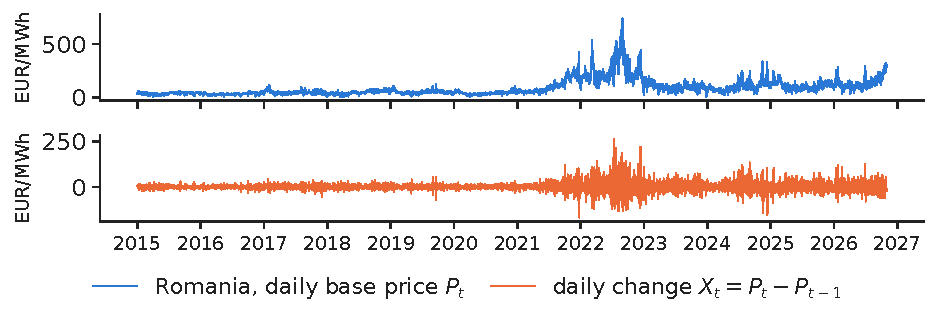
\includegraphics[width=\textwidth,height=0.439\textheight,keepaspectratio]{charts/en/price_changes.pdf}\end{center}\vspace{-3mm}
\chartsource{Source: energy-charts.info (Fraunhofer ISE); OPCOM day-ahead prices for Romania, via ENTSO-E; own estimates. Data: daily, 2015-01-01 to 2026-10-31 (CET delivery days).}
\vspace{0.5mm}
\begin{itemize}\setlength{\itemsep}{0pt}
  \item $X_t=P_t-P_{t-1}$ = change of the daily base price, EUR/MWh
    \begin{itemize}\setlength{\itemsep}{0pt}
      \item Prices can be negative, so we use changes, not log returns
      \item Largest rise 260.77 (11 Jul 2022), largest fall \ensuremath{-}166.59 EUR/MWh (24 Dec 2021)
    \end{itemize}
\end{itemize}
\par\vfill\manager{a supplier that buys 100 MW flat on the PZU and budgets at yesterday's price loses 2,400 EUR for every EUR/MWh of rise.}\par\vspace{0.5mm}
\par\vfill\noindent{\scriptsize\color{FooterGray}(OPCOM; EPEX SPOT; own computation)}\hfill\qlink{EMQA\_L4\_price\_changes}{Quantlets/L4/EMQA_L4_price_changes}\par\vspace{0.5mm}
\end{frame}

\begin{frame}{Value-at-risk is a quantile of tomorrow's loss}
\footnotesize
\intuition{VaR is the loss that is exceeded only on a small, chosen share of days, e.g.\ one day in a hundred.}
\begin{columns}[T,onlytextwidth]
\begin{column}{0.55\textwidth}
\[ \underbrace{L_{t}=Q\cdot 24\cdot X_{t}}_{\text{loss, EUR}},\qquad \underbrace{\text{VaR}_{\alpha,t}=\min\{\ell:\ \Pr(L_t\le \ell\mid\mathcal F_{t-1})\ge\alpha\}}_{\text{the } \alpha\text{-quantile of the loss}} \]{\footnotesize\begin{itemize}\setlength{\itemsep}{0pt}
  \item \textbf{\txtwhere}
    \begin{itemize}\setlength{\itemsep}{0pt}
      \item $Q$ = position in MW (100 MW flat: $Q\cdot 24$ = 2,400 MWh per day)
      \item $X_t$ = price change, EUR/MWh
      \item $\alpha$ = confidence level, 0.95 or 0.99
      \item $\mathcal F_{t-1}$ = information up to day $t-1$ (prices known at 12:00 CET, gate closure).
    \end{itemize}
\end{itemize}\par}
\end{column}
\begin{column}{0.42\textwidth}
\begin{itemize}\setlength{\itemsep}{1pt}
  \item \textbf{On our data}, last 365 days
    \begin{itemize}\setlength{\itemsep}{0pt}
      \item 99\% quantile of $X_t$: 86.63 EUR/MWh, i.e.\ VaR$_{0.99}$ = 207\,922 EUR for 100 MW
      \item 95\% quantile: 50.39 EUR/MWh
    \end{itemize}
  \item \textbf{What VaR does not say}
    \begin{itemize}\setlength{\itemsep}{0pt}
      \item How large the loss is on the worst 1\% of days
      \item For that we need the ES, next slide
    \end{itemize}
\end{itemize}
\end{column}
\end{columns}
\par\vfill\manager{the desk reports the 99\% VaR every morning, before bidding at 12:00 CET.}\par\vspace{0.5mm}
\par\vfill\noindent{\scriptsize\color{FooterGray}(Jorion, 2007; McNeil, Frey \& Embrechts, 2015)}\hfill\tryit{notebook \S2}\par\vspace{0.5mm}
\end{frame}

\begin{frame}{Expected shortfall: the average loss beyond VaR}
\footnotesize
\intuition{When a bad day comes, how large is the loss on average?}
\begin{columns}[T,onlytextwidth]
\begin{column}{0.53\textwidth}
\[ \text{ES}_{\alpha,t}=\E\big[L_t\mid L_t\ge \text{VaR}_{\alpha,t}\big]=\frac{1}{1-\alpha}\int_{\alpha}^{1}\text{VaR}_{u,t}\,du \]\[ \underbrace{\text{ES}(L_1+L_2)\le\text{ES}(L_1)+\text{ES}(L_2)}_{\text{subadditivity: diversification never adds risk}} \]{\footnotesize\begin{itemize}\setlength{\itemsep}{0pt}
  \item \textbf{\txtwhere}
    \begin{itemize}\setlength{\itemsep}{0pt}
      \item ES is coherent, VaR may break subadditivity
      \item The Fundamental Review of the Trading Book (FRTB) uses ES at 97.5\% instead of VaR at 99\%.
    \end{itemize}
\end{itemize}\par}
\end{column}
\begin{column}{0.44\textwidth}
\begin{itemize}\setlength{\itemsep}{1pt}
  \item \textbf{On our data}, last 365 days, EUR/MWh
    \begin{itemize}\setlength{\itemsep}{0pt}
      \item VaR$_{0.975}$ 61.96, ES$_{0.975}$ 86.91 (mean of the 10 worst days)
    \end{itemize}
  \item \textbf{Romania + Germany--Luxembourg}, 100 MW in each
    \begin{itemize}\setlength{\itemsep}{0pt}
      \item 99\% VaR: 86.63 + 91.76 separately, 150.77 together
      \item Correlation 0.55: the joint risk is smaller
    \end{itemize}
\end{itemize}
\end{column}
\end{columns}
\par\vfill\manager{size the cash buffer with ES, not with VaR.}\par\vspace{0.5mm}
\par\vfill\noindent{\scriptsize\color{FooterGray}(Artzner et al., 1999, Math.\ Finance; Acerbi \& Tasche, 2002, JBF; BCBS, 2019)}\hfill\tryit{notebook \S2}\par\vspace{0.5mm}
\end{frame}

\begin{frame}{Large price rises are far more frequent than the normal curve allows}
\small
\begin{center}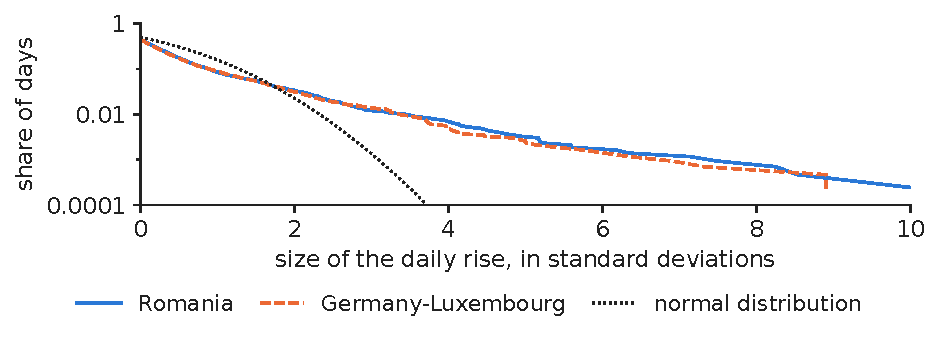
\includegraphics[width=\textwidth,height=0.477\textheight,keepaspectratio]{charts/en/tails.pdf}\end{center}\vspace{-3mm}
\chartsource{Source: energy-charts.info (Fraunhofer ISE); OPCOM (RO) and EPEX SPOT (DE-LU) day-ahead prices, via ENTSO-E. Data: daily changes, 2015-01-01 to 2026-10-31.}
\vspace{0.5mm}
\begin{itemize}\setlength{\itemsep}{0pt}
  \item Excess kurtosis 12.0 in Romania, 12.1 in Germany--Luxembourg (0 for a normal curve)
    \begin{itemize}\setlength{\itemsep}{0pt}
      \item Rises above 3 standard deviations: 52 days observed vs 5.8 expected under normality
      \item The largest rise is 10.1 standard deviations: under normality, once in more than $10^{20}$ years
    \end{itemize}
\end{itemize}
\par\vfill\manager{a limit built on the normal curve understates how often a crisis day comes (Lecture 1).}\par\vspace{0.5mm}
\par\vfill\noindent{\scriptsize\color{FooterGray}(own computation, 1 Jan 2015 -- 31 Oct 2026)}\hfill\qlink{EMQA\_L4\_tails}{Quantlets/L4/EMQA_L4_tails}\par\vspace{0.5mm}
\end{frame}

\begin{frame}{A normal-curve limit set in 2020 was breached 19 times more often than planned in 2021--2022}
\footnotesize
\intuition{A static limit assumes that tomorrow's risk looks like the past; in a crisis it does not.}
\begin{columns}[T,onlytextwidth]
\begin{column}{0.50\textwidth}
\[ \underbrace{\ell_{0.99}=\hat\mu+z_{0.99}\,\hat\sigma}_{\text{normal 99\% limit}},\qquad z_{0.99}=2.326 \]{\footnotesize\begin{itemize}\setlength{\itemsep}{0pt}
  \item \textbf{\txtwhere}
    \begin{itemize}\setlength{\itemsep}{0pt}
      \item $\hat\mu$, $\hat\sigma$ = mean and standard deviation of $X_t$ in 2015--2020
      \item $z_{0.99}$ = 99\% quantile of the standard normal distribution
      \item A correct limit is exceeded on 1\% of days.
    \end{itemize}
\end{itemize}\par}
\end{column}
\begin{column}{0.47\textwidth}
\begin{itemize}\setlength{\itemsep}{1pt}
  \item \textbf{The limit}, from 2\,182 days of 2015--2020
    \begin{itemize}\setlength{\itemsep}{0pt}
      \item $\hat\sigma$ = 10.21, limit = 23.77 EUR/MWh
      \item Already in 2015--2020: 45 breaches vs 21.8 expected
    \end{itemize}
  \item \textbf{Breaches afterwards}
    \begin{itemize}\setlength{\itemsep}{0pt}
      \item 2021--2022: 139 vs 7.3 expected
      \item 2023--2026: 226 vs 14.0 expected (16 times more)
    \end{itemize}
\end{itemize}
\end{column}
\end{columns}
\par\vfill\manager{a limit must move with volatility
    \begin{itemize}\setlength{\itemsep}{0pt}
      \item The next section shows four ways to make it move.
    \end{itemize}}\par\vspace{0.5mm}
\par\vfill\noindent{\scriptsize\color{FooterGray}(own computation; Lecture 1)}\hfill\tryit{notebook \S2}\par\vspace{0.5mm}
\end{frame}


\section{Estimating VaR and ES: four methods}

\subsection{Historical simulation and parametric models}

\begin{frame}{Historical simulation with a one-year window}
\footnotesize
\intuition{Sort the last 365 daily changes; the 4th largest is the 99\% VaR.}
\begin{columns}[T,onlytextwidth]
\begin{column}{0.50\textwidth}
\[ \widehat{\text{VaR}}^{\text{HS}}_{\alpha,t}=\hat q_{\alpha}\big(X_{t-W},\dots,X_{t-1}\big) \]\[ \widehat{\text{ES}}^{\text{HS}}_{\alpha,t}=\text{mean of }\{X_s\ge\widehat{\text{VaR}}^{\text{HS}}_{\alpha,t}\} \]{\footnotesize\begin{itemize}\setlength{\itemsep}{0pt}
  \item \textbf{\txtwhere}
    \begin{itemize}\setlength{\itemsep}{0pt}
      \item $W$ = 365 days (the window)
      \item $\hat q_\alpha$ = empirical quantile
      \item No distribution is assumed.
    \end{itemize}
\end{itemize}\par}
\end{column}
\begin{column}{0.47\textwidth}
\begin{itemize}\setlength{\itemsep}{1pt}
  \item \textbf{On our data}, October 2026
    \begin{itemize}\setlength{\itemsep}{0pt}
      \item VaR$_{0.99}$ 86.63, ES$_{0.975}$ 87.59 EUR/MWh
      \item 2017--2026: exceeded on 2.04\% of days, not 1\%
    \end{itemize}
  \item \textbf{Weakness}
    \begin{itemize}\setlength{\itemsep}{0pt}
      \item A new regime needs months to fill the window
      \item A crisis day counts for 365 days, then drops out at once
    \end{itemize}
\end{itemize}
\end{column}
\end{columns}
\par\vfill\manager{HS is the default in many energy companies, and it lags the market.}\par\vspace{0.5mm}
\par\vfill\noindent{\scriptsize\color{FooterGray}(Jorion, 2007; Christoffersen, 2012)}\hfill\tryit{notebook \S3}\par\vspace{0.5mm}
\end{frame}

\begin{frame}{Parametric VaR: normal and Student-$t$ distributions}
\footnotesize
\intuition{Fit a curve to the last year of changes and read its quantile; the Student-$t$ curve has fatter tails.}
\begin{columns}[T,onlytextwidth]
\begin{column}{0.55\textwidth}
\[ \text{VaR}^{N}_{\alpha}=\mu+\sigma z_\alpha,\qquad \text{ES}^{N}_{\alpha}=\mu+\sigma\frac{\varphi(z_\alpha)}{1-\alpha} \]\[ \text{VaR}^{t}_{\alpha}=m+s\,t_{\nu,\alpha},\qquad \text{ES}^{t}_{\alpha}=m+s\,\frac{g_\nu(t_{\nu,\alpha})}{1-\alpha}\cdot\frac{\nu+t_{\nu,\alpha}^2}{\nu-1} \]{\footnotesize\begin{itemize}\setlength{\itemsep}{0pt}
  \item \textbf{\txtwhere}
    \begin{itemize}\setlength{\itemsep}{0pt}
      \item $\mu,\sigma$ = mean, standard deviation
      \item $z_\alpha$, $\varphi$ = normal quantile, density
      \item $m,s,\nu$ = location, scale, degrees of freedom, by maximum likelihood estimation (MLE)
      \item $t_{\nu,\alpha}$, $g_\nu$ = Student-$t$ quantile, density (Appendix A).
    \end{itemize}
\end{itemize}\par}
\end{column}
\begin{column}{0.42\textwidth}
\begin{itemize}\setlength{\itemsep}{1pt}
  \item \textbf{On our data}, October 2026, EUR/MWh
    \begin{itemize}\setlength{\itemsep}{0pt}
      \item Normal: VaR$_{0.99}$ 69.64, ES$_{0.975}$ 69.98
      \item Student-$t$: VaR$_{0.99}$ 76.66, ES$_{0.975}$ 80.05
    \end{itemize}
  \item \textbf{Backtest}, days above the 99\% VaR
    \begin{itemize}\setlength{\itemsep}{0pt}
      \item Normal 3.21\%, Student-$t$ 1.98\% (target 1\%)
      \item At 95\% the $t$ curve is too narrow: 8.75\%
    \end{itemize}
\end{itemize}
\end{column}
\end{columns}
\par\vfill\manager{the normal VaR is the easiest to explain and the most dangerous to trust.}\par\vspace{0.5mm}
\par\vfill\noindent{\scriptsize\color{FooterGray}(McNeil, Frey \& Embrechts, 2015)}\hfill\tryit{notebook \S3}\par\vspace{0.5mm}
\end{frame}

\subsection{Filtered historical simulation and extreme values}

\begin{frame}{Filtered historical simulation: past shocks rescaled to current volatility}
\footnotesize
\intuition{Divide past changes by their volatility, then rescale the shocks by today's volatility.}
\begin{columns}[T,onlytextwidth]
\begin{column}{0.53\textwidth}
\[ e_t=X_t-\mu_{d(t)},\quad \sigma_t^2=\omega+a\,e_{t-1}^2+b\,\sigma_{t-1}^2,\quad z_t=e_t/\sigma_t \]\[ \text{VaR}^{\text{FHS}}_{\alpha,t}=\mu_{d(t)}+\sigma_t\,\hat q_\alpha(z) \]{\footnotesize\begin{itemize}\setlength{\itemsep}{0pt}
  \item \textbf{\txtwhere}
    \begin{itemize}\setlength{\itemsep}{0pt}
      \item $\mu_{d(t)}$ = mean change of that weekday (prices fall at weekends)
      \item $\sigma_t$ = generalised autoregressive conditional heteroskedasticity (GARCH) volatility, Lecture 3, refitted every 21 days on 730 days
      \item ES: $\sigma_t$ times the mean of $z$ above $\hat q_\alpha(z)$.
    \end{itemize}
\end{itemize}\par}
\end{column}
\begin{column}{0.44\textwidth}
\begin{itemize}\setlength{\itemsep}{1pt}
  \item \textbf{On our data}, GARCH(1,1)
    \begin{itemize}\setlength{\itemsep}{0pt}
      \item $\sigma_t$ from 4.06 (29 Mar 2021) to 100.86 EUR/MWh (12 Jul 2022)
      \item October 2026: VaR$_{0.99}$ 67.50 EUR/MWh
    \end{itemize}
  \item \textbf{Backtest}
    \begin{itemize}\setlength{\itemsep}{0pt}
      \item 99\%: 1.51\% of days
      \item 95\%: 5.58\%, Kupiec $p$ = 0.120
    \end{itemize}
\end{itemize}
\end{column}
\end{columns}
\par\vfill\manager{FHS raises the limit within days of a volatility jump
    \begin{itemize}\setlength{\itemsep}{0pt}
      \item HS needs months.
    \end{itemize}}\par\vspace{0.5mm}
\par\vfill\noindent{\scriptsize\color{FooterGray}(Barone-Adesi, Giannopoulos \& Vosper, 1999; Bollerslev, 1986)}\hfill\tryit{notebook \S3}\par\vspace{0.5mm}
\end{frame}

\begin{frame}{Extreme value theory: model only the tail, with a generalised Pareto curve}
\footnotesize
\intuition{Above a high threshold, the excesses of almost any distribution follow the same two-parameter curve.}
\begin{columns}[T,onlytextwidth]
\begin{column}{0.55\textwidth}
\[ \Pr(Z-u\le y\mid Z>u)\approx 1-\Big(1+\frac{\xi y}{\beta}\Big)^{-1/\xi} \]\[ \text{VaR}_\alpha=u+\frac{\beta}{\xi}\Big[\Big(\frac{n}{N_u}(1-\alpha)\Big)^{-\xi}-1\Big],\quad \text{ES}_\alpha=\frac{\text{VaR}_\alpha+\beta-\xi u}{1-\xi} \]{\footnotesize\begin{itemize}\setlength{\itemsep}{0pt}
  \item \textbf{\txtwhere}
    \begin{itemize}\setlength{\itemsep}{0pt}
      \item Peaks over threshold (POT): $u$ = 90\% quantile of $z$, exceeded by $N_u$ of $n$ residuals
      \item Generalised Pareto distribution (GPD): shape $\xi$ (tail heaviness), scale $\beta$, by MLE
      \item Then multiplied by $\sigma_t$ as in FHS (Appendix B).
    \end{itemize}
\end{itemize}\par}
\end{column}
\begin{column}{0.42\textwidth}
\begin{itemize}\setlength{\itemsep}{1pt}
  \item \textbf{Raw changes}, threshold = 95\% quantile
    \begin{itemize}\setlength{\itemsep}{0pt}
      \item $\hat\xi$ = 0.164: a heavy tail
      \item Moments above order 6.1 do not exist
    \end{itemize}
  \item \textbf{After the GARCH filter}
    \begin{itemize}\setlength{\itemsep}{0pt}
      \item Median $\hat\xi$ = 0.011: the filter absorbs most of the tail
      \item 99\% backtest: 1.37\% of days, the best of five
    \end{itemize}
\end{itemize}
\end{column}
\end{columns}
\par\vfill\manager{use EVT for the one-in-ten-years day that no window contains.}\par\vspace{0.5mm}
\par\vfill\noindent{\scriptsize\color{FooterGray}(Pickands, 1975; McNeil \& Frey, 2000; Chan \& Gray, 2006, IJF)}\hfill\tryit{notebook \S3}\par\vspace{0.5mm}
\end{frame}

\begin{frame}{Above the threshold the Pareto curve fits the data; the normal curve does not}
\small
\begin{center}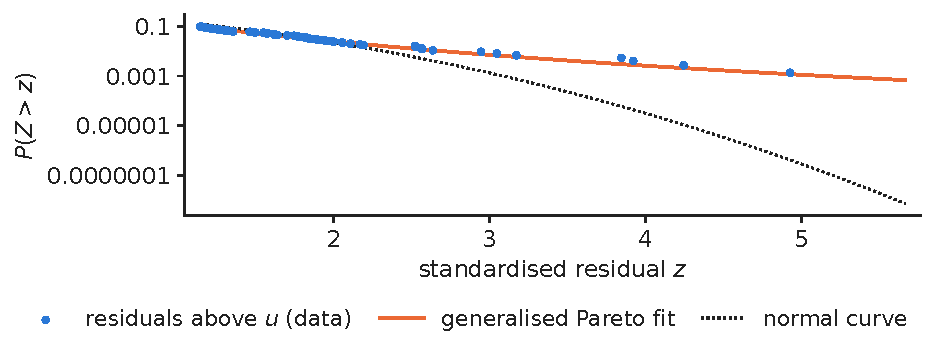
\includegraphics[width=\textwidth,height=0.455\textheight,keepaspectratio]{charts/en/gpd_tail.pdf}\end{center}\vspace{-3mm}
\chartsource{Source: energy-charts.info (Fraunhofer ISE); OPCOM day-ahead prices for Romania, via ENTSO-E; own estimates. Data: GARCH-filtered changes, the 730 days before 2026-10-31.}
\vspace{0.5mm}
\begin{itemize}\setlength{\itemsep}{0pt}
  \item Last refit (11 Oct 2026): $\hat\xi$ = 0.182, $\hat\beta$ = 0.569
    \begin{itemize}\setlength{\itemsep}{0pt}
      \item $\hat\xi>0$ in 53\% of the refits: the standardised tail is sometimes heavy, sometimes not
    \end{itemize}
\end{itemize}
\par\vfill\manager{a 4-sigma day is rare but not impossible
    \begin{itemize}\setlength{\itemsep}{0pt}
      \item The normal curve calls it impossible.
    \end{itemize}}\par\vspace{0.5mm}
\par\vfill\noindent{\scriptsize\color{FooterGray}(Balkema \& de Haan, 1974; McNeil \& Frey, 2000)}\hfill\qlink{EMQA\_L4\_gpd\_tail}{Quantlets/L4/EMQA_L4_gpd_tail}\par\vspace{0.5mm}
\end{frame}

\subsection{Comparing the methods}

\begin{frame}{VaR and ES on the same day by five methods}
\footnotesize
\begin{center}{\footnotesize\renewcommand{\arraystretch}{1.2}\setlength{\tabcolsep}{4pt}
\begin{tabular}{@{}lrrrrr@{}}\toprule
Method & VaR$_{0.95}$ & VaR$_{0.99}$ & ES$_{0.975}$ & VaR$_{0.99}$, kEUR & ES$_{0.975}$, kEUR \\ \midrule
HS & 50.38 & 86.63 & 87.59 & 208 & 210 \\
Normal & 49.33 & 69.64 & 69.98 & 167 & 168 \\
Student-$t$ & 45.77 & 76.66 & 80.05 & 184 & 192 \\
FHS & 36.22 & 67.50 & 67.44 & 162 & 162 \\
EVT & 35.66 & 64.33 & 68.54 & 154 & 164 \\
\bottomrule\end{tabular}}\end{center}\vspace{-1mm}
\par\vspace{0.5mm}{\scriptsize \begin{itemize}\setlength{\itemsep}{0pt}
  \item Mean of the 31 forecasts made for October 2026; first three columns in EUR/MWh; last two for 100 MW flat (2,400 MWh per day).
\end{itemize}}\begin{itemize}\setlength{\itemsep}{1pt}
  \item \textbf{Reading the table}
    \begin{itemize}\setlength{\itemsep}{0pt}
      \item HS and Student-$t$ still carry the volatile days of the past year
      \item FHS and EVT use today's volatility, below the yearly average in October 2026
    \end{itemize}
\end{itemize}
\par\vfill\manager{report two methods side by side and explain the gap.}\par\vspace{0.5mm}
\par\vfill\noindent{\scriptsize\color{FooterGray}(own estimates)}\hfill\tryit{notebook \S3}\par\vspace{0.5mm}
\end{frame}

\begin{frame}{In the crisis FHS adapted within days; HS and the normal VaR lagged}
\small
\begin{center}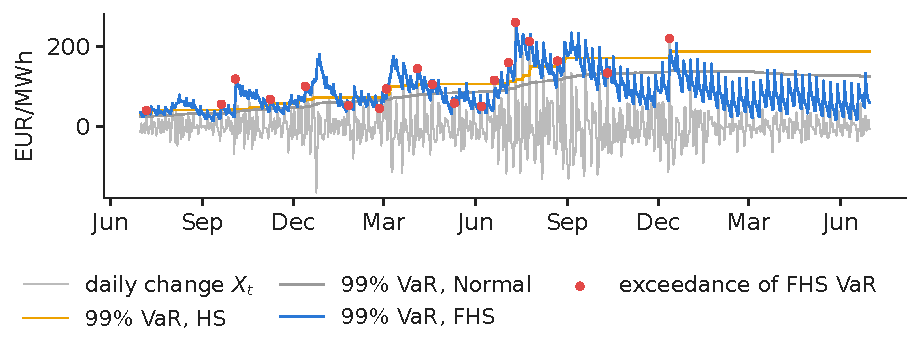
\includegraphics[width=\textwidth,height=0.528\textheight,keepaspectratio]{charts/en/var_paths.pdf}\end{center}\vspace{-3mm}
\chartsource{Source: energy-charts.info (Fraunhofer ISE); OPCOM day-ahead prices for Romania, via ENTSO-E; own estimates. Data: forecasts for 2021-07-01 to 2023-06-30.}
\vspace{0.5mm}
\begin{itemize}\setlength{\itemsep}{0pt}
  \item Exceedances of the 99\% VaR, 1 Jul 2021 -- 30 Jun 2023 (730 days, 7.3 expected)
    \begin{itemize}\setlength{\itemsep}{0pt}
      \item HS 28, normal 45, Student-$t$ 29, FHS 19, EVT 17
    \end{itemize}
\end{itemize}
\par\vfill\manager{in a crisis, a model that reacts within days protects the cash.}\par\vspace{0.5mm}
\par\vfill\noindent{\scriptsize\color{FooterGray}(own estimates)}\hfill\qlink{EMQA\_L4\_var\_paths}{Quantlets/L4/EMQA_L4_var_paths}\par\vspace{0.5mm}
\end{frame}

\begin{frame}{The square-root-of-time rule overstates the 10-day risk}
\small
\begin{center}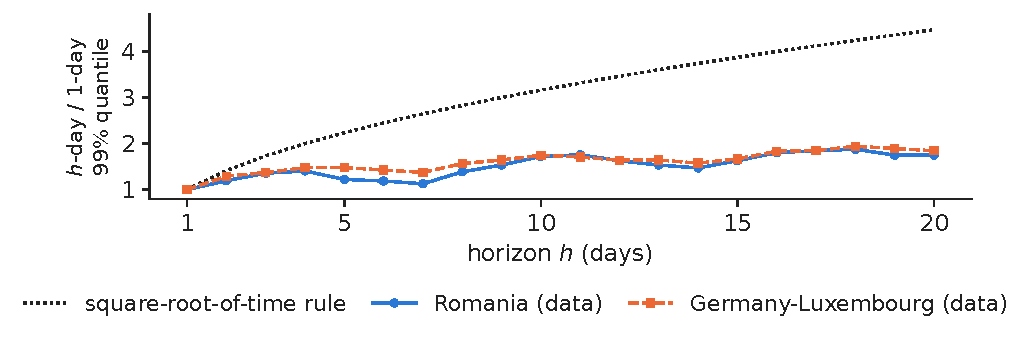
\includegraphics[width=\textwidth,height=0.459\textheight,keepaspectratio]{charts/en/horizon.pdf}\end{center}\vspace{-3mm}
\chartsource{Source: energy-charts.info (Fraunhofer ISE); OPCOM (RO) and EPEX SPOT (DE-LU) day-ahead prices, via ENTSO-E. Data: daily base prices, 2015-01-01 to 2026-10-31.}
\vspace{0.5mm}
\begin{itemize}\setlength{\itemsep}{0pt}
  \item 10-day 99\% quantile = 1.72 $\times$ the 1-day one (RO; 1.75 in DE-LU), not $\sqrt{10}$ = 3.16
    \begin{itemize}\setlength{\itemsep}{0pt}
      \item Variance ratio at 10 days 0.33 (1 = random walk); autocorrelation of $X_t$: \ensuremath{-}0.076 at lag 1, 0.474 at lag 7
    \end{itemize}
\end{itemize}
\par\vfill\manager{for a 10-day horizon, measure 10-day changes directly
    \begin{itemize}\setlength{\itemsep}{0pt}
      \item Multiplying by $\sqrt{10}$ wastes capital.
    \end{itemize}}\par\vspace{0.5mm}
\par\vfill\noindent{\scriptsize\color{FooterGray}(own computation; Weron, 2014, IJF)}\hfill\qlink{EMQA\_L4\_horizon}{Quantlets/L4/EMQA_L4_horizon}\par\vspace{0.5mm}
\end{frame}


\section{Backtesting VaR and ES}

\begin{frame}{Kupiec test of the exceedance frequency}
\footnotesize
\intuition{A 99\% VaR promises to be exceeded on 1\% of days; count the exceedances and test whether the share differs from 1\%.}
\begin{columns}[T,onlytextwidth]
\begin{column}{0.52\textwidth}
\[ I_t=\mathbf 1\{L_t>\text{VaR}_{\alpha,t}\},\qquad x=\textstyle\sum_{t=1}^{n}I_t,\qquad \hat p=x/n \]\[ \text{LR}_{uc}=-2\ln\frac{(1-p)^{n-x}\,p^{x}}{(1-\hat p)^{n-x}\,\hat p^{\,x}}\ \sim\ \chi^2_1 \]{\footnotesize\begin{itemize}\setlength{\itemsep}{0pt}
  \item \textbf{\txtwhere}
    \begin{itemize}\setlength{\itemsep}{0pt}
      \item $I_t$ = exceedance indicator
      \item $p=1-\alpha$ = promised share
      \item Likelihood ratio (LR) test of unconditional coverage
      \item Reject at 5\% if LR$_{uc}>$ 3.84.
    \end{itemize}
\end{itemize}\par}
\end{column}
\begin{column}{0.45\textwidth}
\begin{itemize}\setlength{\itemsep}{1pt}
  \item \textbf{On our data}, 99\% VaR, 3\,587 days
    \begin{itemize}\setlength{\itemsep}{0pt}
      \item Expected 35.9 exceedances
      \item Normal 115, LR$_{uc}$ 111.5; FHS 54, LR$_{uc}$ 8.0
      \item EVT 49, $p$ = 0.037
    \end{itemize}
  \item \textbf{Power of the test}
    \begin{itemize}\setlength{\itemsep}{0pt}
      \item With one year at 99\% we expect only 2--3 exceedances; the test can hardly reject
      \item Ten years of daily data make it sharp
    \end{itemize}
\end{itemize}
\end{column}
\end{columns}
\par\vfill\manager{ask for the exceedance count before you trust anyone's VaR.}\par\vspace{0.5mm}
\par\vfill\noindent{\scriptsize\color{FooterGray}(Kupiec, 1995, J.\ Derivatives)}\hfill\tryit{notebook \S4}\par\vspace{0.5mm}
\end{frame}

\begin{frame}{Christoffersen test of independent exceedances}
\footnotesize
\intuition{A good model is not surprised twice in a row: an exceedance today should not make one tomorrow more likely.}
\begin{columns}[T,onlytextwidth]
\begin{column}{0.55\textwidth}
\[ \pi_{01}=\Pr(I_t=1\mid I_{t-1}=0),\qquad \pi_{11}=\Pr(I_t=1\mid I_{t-1}=1) \]\[ \text{LR}_{ind}=-2\ln\frac{(1-\hat\pi)^{n_{00}+n_{10}}\hat\pi^{\,n_{01}+n_{11}}}{(1-\hat\pi_{01})^{n_{00}}\hat\pi_{01}^{\,n_{01}}(1-\hat\pi_{11})^{n_{10}}\hat\pi_{11}^{\,n_{11}}}\sim\chi^2_1 \]{\footnotesize\begin{itemize}\setlength{\itemsep}{0pt}
  \item \textbf{\txtwhere}
    \begin{itemize}\setlength{\itemsep}{0pt}
      \item $n_{ij}$ = days with $I_{t-1}=i$, $I_t=j$
      \item $\hat\pi$ = overall share
      \item $H_0$: $\pi_{01}=\pi_{11}$
      \item Joint test LR$_{cc}$ = LR$_{uc}$ + LR$_{ind}\sim\chi^2_2$.
    \end{itemize}
\end{itemize}\par}
\end{column}
\begin{column}{0.42\textwidth}
\begin{itemize}\setlength{\itemsep}{1pt}
  \item \textbf{On our data}, 99\% VaR, independence $p$-values
    \begin{itemize}\setlength{\itemsep}{0pt}
      \item HS 0.682, normal 0.868, FHS 0.199
      \item No method fails it: exceedances rarely fall on consecutive days
    \end{itemize}
  \item \textbf{But they cluster in months}
    \begin{itemize}\setlength{\itemsep}{0pt}
      \item Normal: 7.26\% of days in 2021--2022, 2.33\% in 2017--2020
      \item A first-order test misses it; the traffic light sees it
    \end{itemize}
\end{itemize}
\end{column}
\end{columns}
\par\vfill\manager{look at the timing of exceedances, not only at their number.}\par\vspace{0.5mm}
\par\vfill\noindent{\scriptsize\color{FooterGray}(Christoffersen, 1998, IER)}\hfill\tryit{notebook \S4}\par\vspace{0.5mm}
\end{frame}

\begin{frame}{Over ten years only the filtered methods pass at 95\%; at 99\% every method has too many exceedances}
\footnotesize
\begin{center}{\footnotesize\renewcommand{\arraystretch}{1.2}\setlength{\tabcolsep}{4pt}
\begin{tabular}{@{}lrrrrrrr@{}}\toprule
Romania & 95\%: share & Kupiec $p$ & 99\%: count & share, \% & Kupiec $p$ & Christoffersen $p$ & red days, \% \\ \midrule
HS & \cellcolor{Forest!23}6.16 & 0.002 & 73 & \cellcolor{Forest!3}2.04 & $<$0.001 & 0.682 & \cellcolor{Crimson!6}16.7 \\
Normal & \cellcolor{Crimson!10}7.36 & $<$0.001 & 115 & \cellcolor{Crimson!55}3.21 & $<$0.001 & 0.868 & \cellcolor{Crimson!53}29.5 \\
Student-$t$ & \cellcolor{Crimson!48}8.75 & $<$0.001 & 71 & \cellcolor{Forest!6}1.98 & $<$0.001 & 0.630 & \cellcolor{Crimson!12}18.3 \\
FHS & \cellcolor{Forest!39}5.58 & 0.120 & 54 & \cellcolor{Forest!30}1.51 & 0.005 & 0.199 & \cellcolor{Forest!32}6.2 \\
EVT & \cellcolor{Forest!40}5.55 & 0.139 & 49 & \cellcolor{Forest!36}1.37 & 0.037 & 0.244 & \cellcolor{Forest!45}2.8 \\
\bottomrule\end{tabular}}\end{center}\vspace{-1mm}
\par\vspace{0.5mm}{\scriptsize \begin{itemize}\setlength{\itemsep}{0pt}
  \item Backtest 1 Jan 2017 -- 31 Oct 2026; expected: 5\% and 1\% of 3\,587 days (35.9 at 99\%); green = close to the target, red = far.
  \item Red days = share of days whose last 250 days held 10 or more exceedances (next slide); Germany--Luxembourg: Appendix D.
\end{itemize}}
\par\vfill\manager{accept a model at 95\%, but hold extra capital for the 99\% tail that none of them captures fully.}\par\vspace{0.5mm}
\par\vfill\noindent{\scriptsize\color{FooterGray}(Kupiec, 1995; Christoffersen, 1998; own estimates)}\hfill\tryit{notebook \S4}\par\vspace{0.5mm}
\end{frame}

\begin{frame}{The Basel traffic light: the normal VaR spent 30\% of days in the red zone}
\small
\begin{center}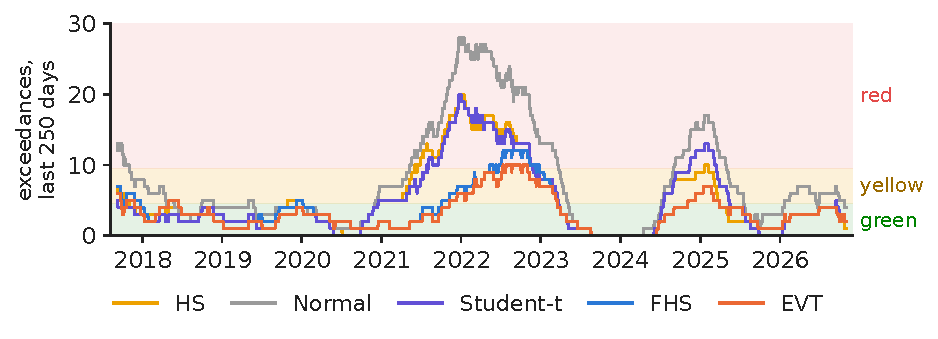
\includegraphics[width=\textwidth,height=0.438\textheight,keepaspectratio]{charts/en/traffic.pdf}\end{center}\vspace{-3mm}
\chartsource{Source: energy-charts.info (Fraunhofer ISE); OPCOM day-ahead prices for Romania, via ENTSO-E; own estimates. Data: backtest 2017-01-01 to 2026-10-31, 99\% VaR.}
\vspace{0.5mm}
\begin{itemize}\setlength{\itemsep}{0pt}
  \item Count of 99\% exceedances in the last 250 days: green 0--4, yellow 5--9, red 10 or more by the Basel Committee on Banking Supervision (BCBS)
    \begin{itemize}\setlength{\itemsep}{0pt}
      \item A correct model is green with probability 89.2\%, red with 0.025\%
      \item Red days: HS 16.7\%, FHS 6.2\%, EVT 2.8\%
    \end{itemize}
\end{itemize}
\par\vfill\manager{yellow means recalibrate, red means stop using the model for limits.}\par\vspace{0.5mm}
\par\vfill\noindent{\scriptsize\color{FooterGray}(BCBS, 1996)}\hfill\qlink{EMQA\_L4\_traffic}{Quantlets/L4/EMQA_L4_traffic}\par\vspace{0.5mm}
\end{frame}

\begin{frame}{Exceedance rates by method in 2021--2022 and since 2023}
\footnotesize
\begin{center}{\footnotesize\renewcommand{\arraystretch}{1.2}\setlength{\tabcolsep}{4pt}
\begin{tabular}{@{}lrrrrrr@{}}\toprule
99\% VaR, \% of days & RO 17--20 & RO 21--22 & RO 23--26 & DE-LU 17--20 & DE-LU 21--22 & DE-LU 23--26 \\ \midrule
HS & \cellcolor{Forest!39}1.58 & \cellcolor{Crimson!53}4.93 & \cellcolor{Forest!55}1.00 & \cellcolor{Forest!51}1.16 & \cellcolor{Crimson!23}3.84 & \cellcolor{Forest!53}1.07 \\
Normal & \cellcolor{Forest!18}2.33 & \cellcolor{Crimson!55}7.26 & \cellcolor{Forest!28}2.00 & \cellcolor{Forest!17}2.40 & \cellcolor{Crimson!55}5.89 & \cellcolor{Forest!26}2.07 \\
Student-$t$ & \cellcolor{Forest!47}1.30 & \cellcolor{Crimson!46}4.66 & \cellcolor{Forest!47}1.29 & \cellcolor{Forest!45}1.37 & \cellcolor{Crimson!27}3.97 & \cellcolor{Forest!47}1.29 \\
FHS & \cellcolor{Forest!45}1.37 & \cellcolor{Forest!3}2.88 & \cellcolor{Forest!53}0.93 & \cellcolor{Forest!43}1.44 & \cellcolor{Forest!15}2.47 & \cellcolor{Forest!45}1.36 \\
EVT & \cellcolor{Forest!48}1.24 & \cellcolor{Forest!15}2.47 & \cellcolor{Forest!53}0.93 & \cellcolor{Forest!41}1.51 & \cellcolor{Forest!22}2.19 & \cellcolor{Forest!53}1.07 \\
\bottomrule\end{tabular}}\end{center}\vspace{-1mm}\begin{itemize}\setlength{\itemsep}{1pt}
  \item \textbf{The crisis}
    \begin{itemize}\setlength{\itemsep}{0pt}
      \item Even FHS was exceeded on 2.88\% of days in Romania: the gas shock moved the whole distribution
    \end{itemize}
  \item \textbf{After the crisis}
    \begin{itemize}\setlength{\itemsep}{0pt}
      \item FHS 0.93\%, EVT 0.93\%, HS 1.00\%, normal 2.00\%
    \end{itemize}
\end{itemize}
\par\vfill\manager{test every model on 2021--2022 before you trust it in a crisis.}\par\vspace{0.5mm}
\par\vfill\noindent{\scriptsize\color{FooterGray}(own estimates)}\hfill\tryit{notebook \S4}\par\vspace{0.5mm}
\end{frame}

\begin{frame}{Backtesting ES: the size of losses beyond VaR}
\footnotesize
\intuition{Divide each exceedance loss by its ES forecast; if ES is right, the ratios average 1.}
\begin{columns}[T,onlytextwidth]
\begin{column}{0.45\textwidth}
\[ Z_2=\frac{1}{T(1-\alpha)}\sum_{t=1}^{T}\frac{L_t\,I_t}{\text{ES}_{\alpha,t}}-1,\qquad \E_{H_0}[Z_2]=0 \]{\footnotesize\begin{itemize}\setlength{\itemsep}{0pt}
  \item \textbf{\txtwhere}
    \begin{itemize}\setlength{\itemsep}{0pt}
      \item $\alpha$ = 0.975
      \item $I_t$ = exceedance of VaR$_{0.975}$
      \item $Z_2>0$ = ES too small
      \item $p$-value from 2,000 paths simulated from each model (Appendix C).
    \end{itemize}
\end{itemize}\par}
\end{column}
\begin{column}{0.52\textwidth}
{\scriptsize\renewcommand{\arraystretch}{1.1}\setlength{\tabcolsep}{4pt}
\begin{tabular}{@{}lrrrrrr@{}}\toprule
$Z_2$ & all & $p$ & 2021--22 & $p$ & 2023--26 & $p$ \\ \midrule
HS & 0.628 & $<$0.001 & 2.694 & $<$0.001 & \ensuremath{-}0.026 & 0.761 \\
Normal & 1.425 & $<$0.001 & 4.170 & $<$0.001 & 0.697 & $<$0.001 \\
Student-$t$ & 0.908 & $<$0.001 & 2.910 & $<$0.001 & 0.329 & 0.052 \\
FHS & 0.335 & 0.004 & 1.164 & $<$0.001 & \ensuremath{-}0.083 & 0.759 \\
EVT & 0.279 & 0.009 & 1.183 & $<$0.001 & \ensuremath{-}0.114 & 0.722 \\
\bottomrule\end{tabular}}\par\vspace{1mm}\begin{itemize}\setlength{\itemsep}{1pt}
  \item \textbf{Reading}: every ES was too small in the crisis
    \begin{itemize}\setlength{\itemsep}{0pt}
      \item Since 2023, FHS, EVT and HS pass.
    \end{itemize}
\end{itemize}
\end{column}
\end{columns}
\par\vfill\manager{judge ES on several years, never on one quarter (about 9 tail days a year).}\par\vspace{0.5mm}
\par\vfill\noindent{\scriptsize\color{FooterGray}(Acerbi \& Székely, 2014; Pele \& Mazurencu-Marinescu-Pele, 2026)}\hfill\tryit{notebook \S4}\par\vspace{0.5mm}
\end{frame}

\begin{frame}{AIDA 2026: a conformal shift measures and corrects the miscalibration of VaR}
\footnotesize
\begin{itemize}\setlength{\itemsep}{1pt}
  \item \textbf{What the work did} (D.\,T.\ Pele, AIDA (AI and Digital Assets in Energy and Finance) conference, 4 June 2026)
    \begin{itemize}\setlength{\itemsep}{0pt}
      \item Score $s_t=\hat q_t-r_t$ ($>0$ on an exceedance day); $\hat q_V$ = 99\% quantile of past scores; corrected VaR = VaR + $\hat q_V$, fixed (audit) or rolling over 250 days
      \item 1\% VaR of 10 models (foundation models, GARCH-type, HS) on 24 assets, incl.\ oil and gas: 240 pairs; Kupiec, Christoffersen, traffic light
    \end{itemize}
  \item \textbf{What it found}
    \begin{itemize}\setlength{\itemsep}{0pt}
      \item $\hat q_V$ from $-$0.007 (too prudent) to +0.102 (no tail signal); it explains 53.4\% (partial $R^2$) of the gain in quantile score
      \item Green-zone pairs: 63/240 (26.2\%) raw, 203/240 (84.6\%) fixed, 234/240 (97.5\%) rolling
      \item The exceedance rate is restored, their clustering is not
    \end{itemize}
  \item \textbf{Link to this lecture}
    \begin{itemize}\setlength{\itemsep}{0pt}
      \item Kupiec says whether VaR fails, $\hat q_V$ by how much; our guarantee widening $\hat c_t$ (Section 4) is the same shift
    \end{itemize}
\end{itemize}
\par\vspace{0.5mm}{\scriptsize \begin{itemize}\setlength{\itemsep}{0pt}
  \item Findings as stated by the authors; talk: \href{https://github.com/danpele/EMQA/blob/main/resources/aida2026/pele_conformal_tail_risk.pdf}{slides}; paper submitted.
\end{itemize}}
\par\vfill\manager{after a failed backtest, widen VaR by the conformal shift and keep testing for clusters.}\par\vspace{0.5mm}
\par\vfill\noindent{\scriptsize\color{FooterGray}(Pele, Bolovăneanu, Ginavar, Lessmann \& Härdle, AIDA, ASE, 4 June 2026)}\par\vspace{0.5mm}
\end{frame}


\section{Margins, guarantees and position limits}

\subsection{Exchange margins}

\begin{frame}{Exchange margins: initial margin as a VaR, variation margin paid daily}
\footnotesize
\intuition{The clearing house holds a deposit that covers a 99\% two-day loss and settles gains and losses in cash every evening.}
\begin{columns}[T,onlytextwidth]
\begin{column}{0.45\textwidth}
\[ \underbrace{\text{IM}_t=K F_t\,\hat q_{0.99}\big(|r^{(2)}|\big)}_{\text{initial margin}},\quad \underbrace{\text{VM}_t=n K(F_t-F_{t-1})}_{\text{variation margin}} \]{\footnotesize\begin{itemize}\setlength{\itemsep}{0pt}
  \item \textbf{\txtwhere}
    \begin{itemize}\setlength{\itemsep}{0pt}
      \item Initial margin (IM), variation margin (VM), set by the central counterparty (CCP)
      \item $F_t$ = futures price
      \item $K$ = 1,000 barrels per Brent lot
      \item $r^{(2)}$ = two-day return
      \item $n$ = lots sold (+) or bought ($-$).
    \end{itemize}
\end{itemize}\par}
\end{column}
\begin{column}{0.52\textwidth}
\begin{itemize}\setlength{\itemsep}{1pt}
  \item \textbf{European Market Infrastructure Regulation (EMIR)}, regulatory technical standards (RTS) 153/2013
    \begin{itemize}\setlength{\itemsep}{0pt}
      \item Futures: 99\%, 2-day liquidation, at least 12 months of data (Art.~24--26)
      \item Anti-procyclicality (APC), Art.~28: a 25\% buffer, or 25\% weight on stress, or a 10-year floor
    \end{itemize}
  \item \textbf{Intercontinental Exchange (ICE) Brent}, 100 lots sold: largest one-day VM 0.88 million USD (16 Sep 2019)
\end{itemize}
\end{column}
\end{columns}
\par\vfill\manager{a hedged producer gains on the physical sale later, but pays the margin today.}\par\vspace{0.5mm}
\par\vfill\noindent{\scriptsize\color{FooterGray}(EU Delegated Regulation 153/2013; ICE Futures Europe)}\hfill\tryit{notebook \S5}\par\vspace{0.5mm}
\end{frame}

\begin{frame}{Margin calls and liquidity shortfalls of hedged energy companies in 2022}
\footnotesize
\begin{itemize}\setlength{\itemsep}{1pt}
  \item \textbf{What happened}, according to the European Central Bank (ECB), November 2022
    \begin{itemize}\setlength{\itemsep}{0pt}
      \item TTF gas futures reached 227 EUR/MWh on 7 March 2022, about 12 times the level of early 2021
      \item By mid-2022 about twice as much initial margin was posted as in late 2021
      \item The firms hurt were mostly utilities and producers that had sold forward: hedgers, not speculators
    \end{itemize}
  \item \textbf{How the European Union (EU) responded}
    \begin{itemize}\setlength{\itemsep}{0pt}
      \item Delegated Regulation (EU) 2022/2311: public guarantees accepted as collateral until 29 November 2023
    \end{itemize}
  \item \textbf{In Romania}, on the day-ahead market
    \begin{itemize}\setlength{\itemsep}{0pt}
      \item OPCOM accepts a buy order at a positive price only up to the participant's guarantee (a bank letter)
    \end{itemize}
\end{itemize}
\par\vfill\manager{the risk that sinks a hedged company is liquidity, not the price itself.}\par\vspace{0.5mm}
\par\vfill\noindent{\scriptsize\color{FooterGray}(ECB, 2022; Delegated Regulation (EU) 2022/2311; OPCOM, 2025)}\par\vspace{0.5mm}
\end{frame}

\begin{frame}{Margins are procyclical: in 2026 the Brent margin rose 2.7-fold in two months}
\small
\begin{center}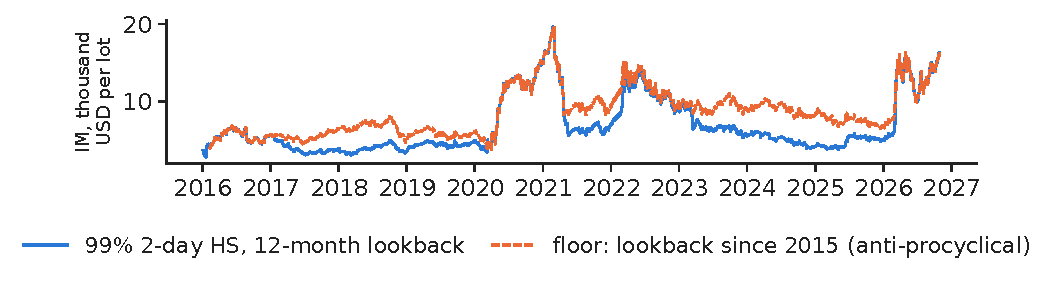
\includegraphics[width=\textwidth,height=0.480\textheight,keepaspectratio]{charts/en/brent_im.pdf}\end{center}\vspace{-3mm}
\chartsource{Source: Yahoo Finance (ICE Brent front-month BZ=F); own computation. Data: trading days 2016-01-01 to 2026-10-30; contract-roll days dropped; 1 lot = 1,000 bbl.}
\vspace{0.5mm}
\begin{itemize}\setlength{\itemsep}{0pt}
  \item Brent rose from 72.48 USD (27 Feb 2026) to 118.35 USD (31 Mar 2026)
    \begin{itemize}\setlength{\itemsep}{0pt}
      \item IM with 12 months of history: 5\,970 $\to$ 16\,313 USD per lot; with the floor since 2015: $\times$2.07 instead of $\times$2.73
      \item Losses beyond IM: 1.80\% of days with 12 months, 0.66\% with the floor (target 1\%)
    \end{itemize}
\end{itemize}
\par\vfill\manager{plan your cash for the margin a crisis would demand, not for today's margin.}\par\vspace{0.5mm}
\par\vfill\noindent{\scriptsize\color{FooterGray}(own computation; EMIR RTS, Art.~28; ICE Brent)}\hfill\qlink{EMQA\_L4\_brent\_im}{Quantlets/L4/EMQA_L4_brent_im}\par\vspace{0.5mm}
\end{frame}

\subsection{Guarantees and limits}

\begin{frame}{The day-ahead guarantee is set from a quantile forecast of tomorrow's price}
\footnotesize
\intuition{To be sure its order clears, a supplier bids up to a high price, and the guarantee must cover price times volume.}
\begin{columns}[T,onlytextwidth]
\begin{column}{0.55\textwidth}
\[ G_t\ \ge\ Q\cdot 24\cdot \hat q_{\tau,t},\qquad \hat q_{\tau,t}=\beta_0+\beta_1P_{t-1}+\beta_2P_{t-7}+\textstyle\sum_j\delta_jD_{j,t} \]\[ \tilde q_{\tau,t}=\hat q_{\tau,t}+\hat c_t,\qquad \hat c_t=\hat q_\tau\big(P_s-\hat q_{\tau,s},\ s=t-365,\dots,t-1\big) \]{\footnotesize\begin{itemize}\setlength{\itemsep}{0pt}
  \item \textbf{\txtwhere}
    \begin{itemize}\setlength{\itemsep}{0pt}
      \item $G_t$ = guarantee, EUR
      \item $\hat q_{\tau,t}$ = quantile regression (QR) on the last 365 days, as in quantile regression averaging (QRA), Lecture 2
      \item $D_{j,t}$ = weekday dummies
      \item $\hat c_t$ = conformal correction from past errors.
    \end{itemize}
\end{itemize}\par}
\end{column}
\begin{column}{0.42\textwidth}
\begin{itemize}\setlength{\itemsep}{1pt}
  \item \textbf{On our data}, $\tau$ = 0.99, 2017--2026
    \begin{itemize}\setlength{\itemsep}{0pt}
      \item Days with the price below the forecast: QR 96.90\%, widened 98.47\%, FHS 98.49\%
    \end{itemize}
  \item \textbf{Cost}, 100 MW flat
    \begin{itemize}\setlength{\itemsep}{0pt}
      \item 0.371 million EUR per day on average, +7.5\% for the widening
      \item 2017--2020: 0.172; 2021--2022: 0.649 million EUR per day
    \end{itemize}
\end{itemize}
\end{column}
\end{columns}
\par\vfill\manager{size the bank line behind the guarantee on the crisis quantile, before the crisis.}\par\vspace{0.5mm}
\par\vfill\noindent{\scriptsize\color{FooterGray}(OPCOM, 2025; Koenker \& Bassett, 1978; Romano et al., 2019)}\hfill\tryit{notebook \S6}\par\vspace{0.5mm}
\end{frame}

\begin{frame}{Heavier tails bring the 99\% quantile close to its nominal coverage}
\small
\begin{center}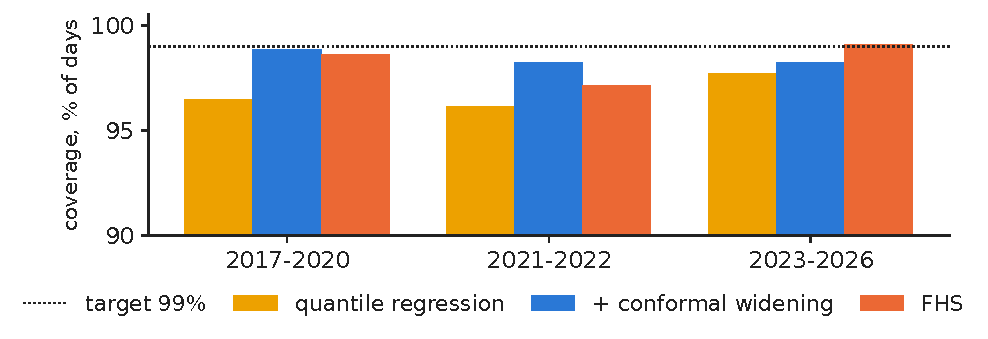
\includegraphics[width=\textwidth,height=0.500\textheight,keepaspectratio]{charts/en/coverage.pdf}\end{center}\vspace{-3mm}
\chartsource{Source: energy-charts.info (Fraunhofer ISE); OPCOM day-ahead prices for Romania, via ENTSO-E; own estimates. Data: forecasts 2017-01-01 to 2026-10-31, 99\% quantile.}
\vspace{0.5mm}
\begin{itemize}\setlength{\itemsep}{0pt}
  \item Kupiec $p$ at 99\%: QR $<$0.001, widened 0.003, FHS 0.005
    \begin{itemize}\setlength{\itemsep}{0pt}
      \item At 95\% the widened QR passes ($p$ = 0.053), as Lecture 2 suggested for the tails
    \end{itemize}
\end{itemize}
\par\vfill\manager{a forecast used for collateral must be calibrated in the tail, not only accurate on average.}\par\vspace{0.5mm}
\par\vfill\noindent{\scriptsize\color{FooterGray}(Nowotarski \& Weron, 2018, RSER; Romano et al., 2019)}\hfill\qlink{EMQA\_L4\_coverage}{Quantlets/L4/EMQA_L4_coverage}\par\vspace{0.5mm}
\end{frame}

\begin{frame}{A position limit in MW should shrink when VaR grows}
\footnotesize
\intuition{The board sets a daily risk budget in EUR; the desk divides it by today's VaR per MW.}
\begin{columns}[T,onlytextwidth]
\begin{column}{0.46\textwidth}
\[ Q^{\max}_t=\frac{B}{24\cdot\text{VaR}^{\text{FHS}}_{0.99,t}} \]{\footnotesize\begin{itemize}\setlength{\itemsep}{0pt}
  \item \textbf{\txtwhere}
    \begin{itemize}\setlength{\itemsep}{0pt}
      \item $B$ = daily VaR budget, here 250,000 EUR (an assumption for the example)
      \item VaR in EUR/MWh
      \item $Q^{\max}_t$ in MW of open flat position.
    \end{itemize}
\end{itemize}\par}
\end{column}
\begin{column}{0.51\textwidth}
\begin{itemize}\setlength{\itemsep}{1pt}
  \item \textbf{On our data}, FHS 99\% VaR
    \begin{itemize}\setlength{\itemsep}{0pt}
      \item 2019 (median): VaR 20.27 EUR/MWh, limit 514 MW
      \item 12 Jul 2022: VaR 245.80, limit 42 MW
      \item 31 Oct 2026: VaR 53.15, limit 196 MW
    \end{itemize}
  \item \textbf{Why it matters}
    \begin{itemize}\setlength{\itemsep}{0pt}
      \item A fixed MW limit lets the money at risk grow with volatility
      \item A fixed EUR budget keeps it constant
    \end{itemize}
\end{itemize}
\end{column}
\end{columns}
\par\vfill\manager{set limits in EUR of VaR and convert them to MW every day.}\par\vspace{0.5mm}
\par\vfill\noindent{\scriptsize\color{FooterGray}(own estimates)}\hfill\tryit{notebook \S6}\par\vspace{0.5mm}
\end{frame}


\section{Price risk for suppliers and producers}

\begin{frame}{A supplier's monthly cost-at-risk under the normal distribution}
\footnotesize
\intuition{A supplier prices next month at this month's cost; the risk is a jump of the load-weighted price.}
\begin{columns}[T,onlytextwidth]
\begin{column}{0.52\textwidth}
\[ \bar P^{L}_m=\frac{\sum_h P_hL_h}{\sum_h L_h},\qquad o_m=\frac{\bar P^{L}_m}{\bar P^{L}_{m-1}}-1 \]\vspace{-2mm}\[ \text{CFaR}_{0.95}=\hat q_{0.95}(o_m) \]{\footnotesize\begin{itemize}\setlength{\itemsep}{0pt}
  \item \textbf{\txtwhere}
    \begin{itemize}\setlength{\itemsep}{0pt}
      \item $P_h$ = hourly price
      \item $L_h$ = Romanian load (portfolio shape)
      \item $o_m$ = cost overrun
      \item Cash-flow-at-risk (CFaR) = its quantile
      \item In EUR for 100 MW on average.
    \end{itemize}
\end{itemize}\par}
\end{column}
\begin{column}{0.45\textwidth}
\begin{itemize}\setlength{\itemsep}{1pt}
  \item \textbf{On our data}, 140 months, Mar 2015 -- Oct 2026
    \begin{itemize}\setlength{\itemsep}{0pt}
      \item Normal 99\% limit (2015--2020): +50.5\%, exceeded 3 times since 2021 (0.7 expected)
      \item Worst month Nov 2024: +86.6\%, 5.96 million EUR
    \end{itemize}
  \item \textbf{Empirical, all months}
    \begin{itemize}\setlength{\itemsep}{0pt}
      \item CFaR$_{0.95}$ = +39.9\%, i.e.\ 2.84 million EUR
      \item ES$_{0.95}$ = +60.2\%, i.e.\ 6.49 million EUR
    \end{itemize}
\end{itemize}
\end{column}
\end{columns}
\par\vfill\manager{price a fixed retail offer with an ES-based premium, or hedge it forward (Lecture 5).}\par\vspace{0.5mm}
\par\vfill\noindent{\scriptsize\color{FooterGray}(own computation; Assignment 2)}\hfill\tryit{notebook \S7}\par\vspace{0.5mm}
\end{frame}

\begin{frame}{Since 2021 the normal 99\% monthly limit was exceeded 3 times (0.7 expected)}
\small
\begin{center}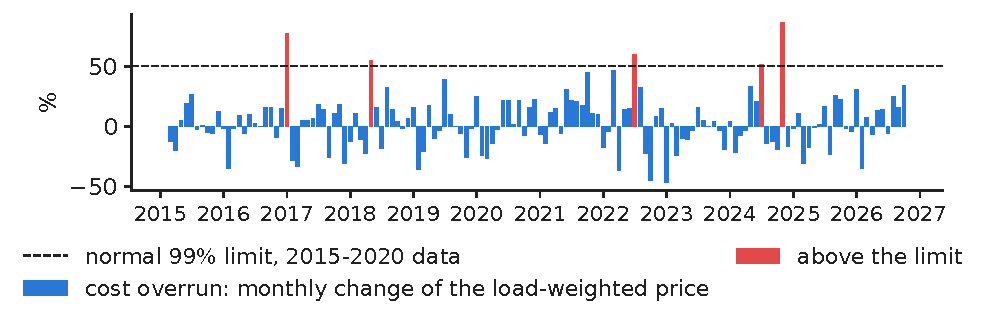
\includegraphics[width=\textwidth,height=0.520\textheight,keepaspectratio]{charts/en/supplier_month.pdf}\end{center}\vspace{-3mm}
\chartsource{Source: energy-charts.info (Fraunhofer ISE); OPCOM prices; ENTSO-E load (Transelectrica data for Romania). Data: monthly, 2015-03 to 2026-10.}
\vspace{0.5mm}
\begin{itemize}\setlength{\itemsep}{0pt}
  \item Red bars exceed the limit computed in 2020
    \begin{itemize}\setlength{\itemsep}{0pt}
      \item The largest overrun came in Nov 2024, after the summer of 2024.
    \end{itemize}
\end{itemize}
\par\vfill\manager{re-estimate the monthly limit every quarter and stress it with the 2022 months.}\par\vspace{0.5mm}
\par\vfill\noindent{\scriptsize\color{FooterGray}(own computation)}\hfill\qlink{EMQA\_L4\_supplier\_month}{Quantlets/L4/EMQA_L4_supplier_month}\par\vspace{0.5mm}
\end{frame}

\begin{frame}{Loss tails: the supplier's tail is heavier than the producer's}
\footnotesize
\intuition{A supplier loses when the price rises, a producer when it falls; prices jump up more than down.}
\begin{columns}[T,onlytextwidth]
\begin{column}{0.47\textwidth}
\[ L^{\text{buyer}}_t=+Q\,24\,X_t,\qquad L^{\text{seller}}_t=-Q\,24\,X_t \]{\footnotesize\begin{itemize}\setlength{\itemsep}{0pt}
  \item \textbf{\txtwhere}
    \begin{itemize}\setlength{\itemsep}{0pt}
      \item One distribution of $X_t$, two tails: upper (supplier), lower (producer selling spot)
      \item Skewness of $X_t$: 1.02.
    \end{itemize}
\end{itemize}\par}
\end{column}
\begin{column}{0.50\textwidth}
\begin{itemize}\setlength{\itemsep}{1pt}
  \item \textbf{Daily}, EUR/MWh, 1 Jan 2015 -- 31 Oct 2026
    \begin{itemize}\setlength{\itemsep}{0pt}
      \item 99\% quantile (supplier): +88.21; 1\% quantile (producer): \ensuremath{-}70.74
      \item ES$_{0.975}$: 91.29 (supplier) vs 74.92 (producer)
    \end{itemize}
  \item \textbf{Monthly base price}
    \begin{itemize}\setlength{\itemsep}{0pt}
      \item 95\% quantile of the change +42.4\%, 5\% quantile \ensuremath{-}32.3\%
    \end{itemize}
\end{itemize}
\end{column}
\end{columns}
\par\vfill\manager{the producer's price risk is smaller, but a dry year adds volume risk (next slide).}\par\vspace{0.5mm}
\par\vfill\noindent{\scriptsize\color{FooterGray}(own computation)}\hfill\tryit{notebook \S7}\par\vspace{0.5mm}
\end{frame}

\begin{frame}{Case study C4: a systemic risk meter and two risks specific to energy companies}
\footnotesize
\begin{itemize}\setlength{\itemsep}{1pt}
  \item \textbf{The paper} (Toma, Dima, Grecu, Pele \& Lessmann, 2026)
    \begin{itemize}\setlength{\itemsep}{0pt}
      \item Data and method: 100 European energy companies, 2016--2026; 5\% quantile regressions with the least absolute shrinkage and selection operator (LASSO); the mean penalty is the Energy Financial Risk Meter (EFRM)
      \item Result: the EFRM captures 2020 and 2022; with the ECB's Composite Indicator of Systemic Stress (CISS) it predicts volatile months with area under the curve (AUC) 0.731
    \end{itemize}
  \item \textbf{Our replication} on three Romanian companies (OMV Petrom, Romgaz, Nuclearelectrica)
    \begin{itemize}\setlength{\itemsep}{0pt}
      \item AUC 0.38, against 0.61 for past volatility: a systemic meter needs many firms, as in the paper
    \end{itemize}
  \item \textbf{Energy-specific risks}
    \begin{itemize}\setlength{\itemsep}{0pt}
      \item Price--volume premium of the household profile: 5.2\% of the base price in 2025
      \item Dry-year buy-back of a hydro fleet that sold its median output forward: 394 million EUR (2022)
    \end{itemize}
\end{itemize}
\par\vfill\manager{put the systemic meter, the price--volume premium and the dry-year cost on one dashboard.}\par\vspace{0.5mm}
\par\vfill\noindent{\scriptsize\color{FooterGray}(Toma, Dima, Grecu, Pele \& Lessmann, 2026, SSRN; case study C4)}\par\vspace{0.5mm}
\end{frame}

\begin{frame}{AIDA 2026: systemic tail risk in EU energy broke upward in July 2021}
\footnotesize
\begin{itemize}\setlength{\itemsep}{1pt}
  \item \textbf{What the work did} (F.-M.\ Toma, AIDA conference, 3 June 2026; paper of case study C4)
    \begin{itemize}\setlength{\itemsep}{0pt}
      \item 100 European energy firms, April 2016 -- March 2026: each firm's 5\% return quantile regressed by LASSO on the other 99 firms, oil, gas and stock indices
      \item EFRM = mean LASSO penalty: more links needed to explain the tail = more systemic exposure
    \end{itemize}
  \item \textbf{What it found}
    \begin{itemize}\setlength{\itemsep}{0pt}
      \item EFRM breaks: February 2020 (pandemic) and July 2021 (gas run-up), seven months before the invasion
      \item Geopolitical risk moved the EFRM only after the invasion: +1.52 percentage points (time-varying model)
      \item Effect on Stoxx 600 stocks about 60\% weaker since, on 5-year credit default swaps still positive
      \item Volatile months: AUC 0.731 for EFRM + CISS, 0.708 EFRM alone, 0.673 CISS alone
    \end{itemize}
\end{itemize}
\par\vspace{0.5mm}{\scriptsize \begin{itemize}\setlength{\itemsep}{0pt}
  \item Findings as stated by the authors; talk: \href{https://github.com/danpele/EMQA/blob/main/resources/aida2026/toma_energy_financial_risk_meter.pdf}{slides}; paper: \href{https://doi.org/10.2139/ssrn.6985301}{doi:10.2139/ssrn.6985301}.
\end{itemize}}
\par\vfill\manager{a firm's own VaR cannot see contagion
    \begin{itemize}\setlength{\itemsep}{0pt}
      \item Read a sector meter next to it.
    \end{itemize}}\par\vspace{0.5mm}
\par\vfill\noindent{\scriptsize\color{FooterGray}(Toma, AIDA, ASE, 3 June 2026; Toma, Dima, Grecu, Pele \& Lessmann, 2026, SSRN)}\par\vspace{0.5mm}
\end{frame}

\begin{frame}{AIDA 2026: the tail risk of carbon-heavy firms predicts the low-carbon premium}
\footnotesize
\begin{itemize}\setlength{\itemsep}{1pt}
  \item \textbf{What the work did} (Prof.\ Wolfgang Karl Härdle, AIDA, 5 June 2026; with R.\ Wang and L.\ Zhang)
    \begin{itemize}\setlength{\itemsep}{0pt}
      \item Carbon premium puzzle: do high-carbon firms earn more (risk compensation) or low-carbon firms (green preference)?
      \item China, July 2014 -- February 2025: 50 high-carbon and 50 low-carbon firms; LASSO regressions as for the EFRM, 63 days, 5\% quantile
      \item Carbon risk dynamic indicator (CARDI) = Financial Risk Meter (FRM, mean penalty $\lambda$), high-carbon / low-carbon firms
    \end{itemize}
  \item \textbf{What it found}
    \begin{itemize}\setlength{\itemsep}{0pt}
      \item High-risk regimes of CARDI coincide with unexpected or early-stage climate-policy events
      \item A rising CARDI predicts a higher factor-adjusted low-carbon premium next month (0.022, 118 months); the conditional VaR ratio does not
      \item Long low-carbon, short high-carbon only when CARDI rises (2015--2024): 115.84\%, Sharpe 0.72 (always on: 89.03\%, 0.49)
    \end{itemize}
  \item \textbf{Link to this lecture}: the EFRM of the previous frame, split by carbon intensity
\end{itemize}
\par\vspace{0.5mm}{\scriptsize \begin{itemize}\setlength{\itemsep}{0pt}
  \item Findings as stated by the authors; talk: \href{https://github.com/danpele/EMQA/blob/main/resources/aida2026/wang_carbon_risk_dynamics.pdf}{slides}; paper: \href{https://doi.org/10.2139/ssrn.5757742}{doi:10.2139/ssrn.5757742}.
\end{itemize}}
\par\vfill\manager{in an oil and gas firm, watch CARDI: when it rises, investors favour low-carbon peers.}\par\vspace{0.5mm}
\par\vfill\noindent{\scriptsize\color{FooterGray}(Wang, Härdle \& Zhang, AIDA, ASE, 5 June 2026; 2025, SSRN)}\par\vspace{0.5mm}
\end{frame}


\section{Case study: the price rise of autumn 2026}

\begin{frame}{Case study: in 2026 the price doubled gradually, without jumps}
\small
\begin{center}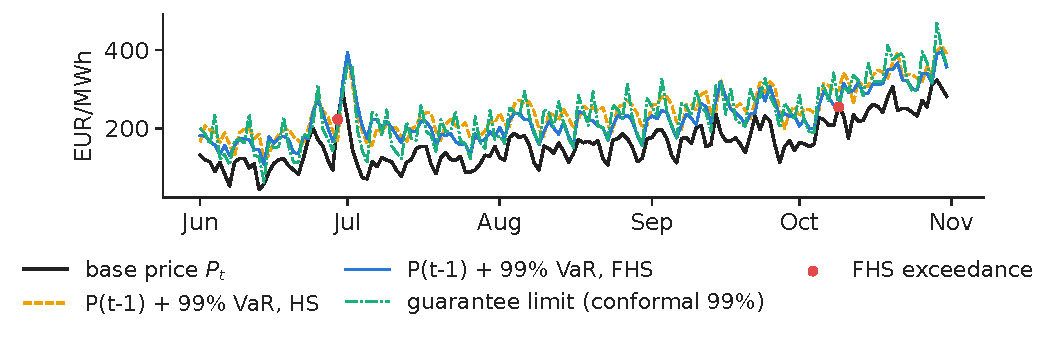
\includegraphics[width=\textwidth,height=0.520\textheight,keepaspectratio]{charts/en/case2026.pdf}\end{center}\vspace{-3mm}
\chartsource{Source: energy-charts.info (Fraunhofer ISE); OPCOM day-ahead prices for Romania, via ENTSO-E; own estimates. Data: daily, 2026-06-01 to 2026-10-31.}
\vspace{0.5mm}
\begin{itemize}\setlength{\itemsep}{0pt}
  \item Monthly mean 122.99 EUR/MWh in June, 239.32 in October; peak 323.76 (29 Oct 2026)
    \begin{itemize}\setlength{\itemsep}{0pt}
      \item 99\% VaR exceedances in 153 days (1.5 expected): FHS 2, HS 1, normal 3
    \end{itemize}
\end{itemize}
\par\vfill\manager{a slow rise passes the VaR tests and still drains cash: watch the price level too.}\par\vspace{0.5mm}
\par\vfill\noindent{\scriptsize\color{FooterGray}(own estimates; OPCOM)}\hfill\qlink{EMQA\_L4\_case2026}{Quantlets/L4/EMQA_L4_case2026}\par\vspace{0.5mm}
\end{frame}

\begin{frame}{Case study: market risk and liquidity needs in 2026}
\footnotesize
\begin{columns}[T,onlytextwidth]
\begin{column}{0.50\textwidth}
\begin{itemize}\setlength{\itemsep}{1pt}
  \item \textbf{Market risk barely moved}
    \begin{itemize}\setlength{\itemsep}{0pt}
      \item FHS 99\% VaR: 61.64 EUR/MWh in June, 67.50 in October
      \item ES test since 2023, FHS: $Z_2$ = \ensuremath{-}0.083, not rejected
    \end{itemize}
  \item \textbf{Cash needs doubled}
    \begin{itemize}\setlength{\itemsep}{0pt}
      \item Day-ahead guarantee for 100 MW (widened 99\% quantile): 0.416 $\to$ 0.776 million EUR per day
      \item Orders above the guarantee limit: 3 days (6 without widening)
    \end{itemize}
\end{itemize}
\end{column}
\begin{column}{0.47\textwidth}
\begin{itemize}\setlength{\itemsep}{1pt}
  \item \textbf{The supplier's monthly bill}, 100 MW
    \begin{itemize}\setlength{\itemsep}{0pt}
      \item August +25.1\% (2.38 million EUR), September +16.2\% (1.86), October +34.0\% (4.68)
      \item Each month below the 99\% limit of +50.5\%, but three in a row
    \end{itemize}
  \item \textbf{Drivers}
    \begin{itemize}\setlength{\itemsep}{0pt}
      \item TTF gas 44.94 $\to$ 86.81 EUR/MWh (June $\to$ October)
      \item Brent 108.34 USD in October; Germany--Luxembourg 169.48 EUR/MWh
    \end{itemize}
\end{itemize}
\end{column}
\end{columns}
\par\vfill\manager{a risk report needs a liquidity line next to VaR: guarantees, margins and the cumulative monthly overrun.}\par\vspace{0.5mm}
\par\vfill\noindent{\scriptsize\color{FooterGray}(own estimates; OPCOM; World Bank; Yahoo Finance)}\hfill\tryit{notebook \S8}\par\vspace{0.5mm}
\end{frame}

\begin{frame}{A risk desk checklist for energy prices}
\footnotesize
\begin{columns}[T,onlytextwidth]
\begin{column}{0.49\textwidth}
\begin{itemize}\setlength{\itemsep}{1pt}
  \item \textbf{Measure}
    \begin{itemize}\setlength{\itemsep}{0pt}
      \item Define the position and the sign of the loss (buyer or seller)
      \item Use only data known at gate closure
      \item Report VaR and ES from two methods, one of them filtered (FHS or EVT)
    \end{itemize}
  \item \textbf{Check}
    \begin{itemize}\setlength{\itemsep}{0pt}
      \item Kupiec, Christoffersen and the traffic light on several years, including 2021--2022
      \item $Z_2$ for ES; never rank models on a few tail days
    \end{itemize}
\end{itemize}
\end{column}
\begin{column}{0.48\textwidth}
\begin{itemize}\setlength{\itemsep}{1pt}
  \item \textbf{Decide}
    \begin{itemize}\setlength{\itemsep}{0pt}
      \item Limits in EUR of VaR, converted daily to MW
      \item Guarantees and credit lines from calibrated high quantiles
      \item A cash buffer for the margin a crisis would demand
    \end{itemize}
  \item \textbf{Report}
    \begin{itemize}\setlength{\itemsep}{0pt}
      \item In EUR and in MW, by month, with the liquidity next to the market risk
    \end{itemize}
\end{itemize}
\end{column}
\end{columns}
\par\vfill\manager{Assignment 2 (Task 5) applies this checklist to the cash flow of your own role.}\par\vspace{0.5mm}
\par\vfill\noindent{\scriptsize\color{FooterGray}(BCBS, 2019; EMIR RTS 153/2013; Assignment 2)}\par\vspace{0.5mm}
\end{frame}

\section*{Wrap-up}

\begin{frame}{Quiz 1: reading a VaR}
\small
\begin{itemize}
  \item Your 99\% one-day VaR for 100 MW is 162 thousand EUR
    \begin{itemize}\setlength{\itemsep}{0pt}
      \item What does it promise, and what does it not say?
    \end{itemize}
\end{itemize}
\vspace{2mm}
\begin{exampleblock}{Answer}
\begin{itemize}
  \item On about 1 day in 100 the loss should exceed it
    \begin{itemize}\setlength{\itemsep}{0pt}
      \item It says nothing about how large the loss is on those days, which is what ES (162 thousand EUR at 97.5\%) measures.
    \end{itemize}
\end{itemize}
\end{exampleblock}
\end{frame}

\begin{frame}{Quiz 2: seven exceedances}
\small
\begin{itemize}
  \item Over the last 250 days your 99\% VaR was exceeded 7 times
    \begin{itemize}\setlength{\itemsep}{0pt}
      \item What zone is it in, and what does Kupiec say?
    \end{itemize}
\end{itemize}
\vspace{2mm}
\begin{exampleblock}{Answer}
\begin{itemize}
  \item Yellow (5--9)
    \begin{itemize}\setlength{\itemsep}{0pt}
      \item LR$_{uc}$ = 5.50, $p$ = 0.019: rejected at 5\%
      \item Recalibrate (e.g.\ move from HS to FHS) and keep watching.
    \end{itemize}
\end{itemize}
\end{exampleblock}
\end{frame}

\begin{frame}{Quiz 3: ten-day VaR}
\small
\begin{itemize}
  \item Your chief financial officer computes the 10-day VaR as $\sqrt{10}$ times the 1-day VaR
    \begin{itemize}\setlength{\itemsep}{0pt}
      \item Is that prudent or wasteful for power?
    \end{itemize}
\end{itemize}
\vspace{2mm}
\begin{exampleblock}{Answer}
\begin{itemize}
  \item Wasteful: power prices revert, and the empirical 10-day 99\% quantile is only 1.72 times the 1-day one in Romania, not 3.16.
\end{itemize}
\end{exampleblock}
\end{frame}

\begin{frame}{Quiz 4: a margin call}
\small
\begin{itemize}
  \item You sold 100 lots of Brent to hedge your production
    \begin{itemize}\setlength{\itemsep}{0pt}
      \item Today the price rises by 5 USD per barrel
      \item What happens tonight?
    \end{itemize}
\end{itemize}
\vspace{2mm}
\begin{exampleblock}{Answer}
\begin{itemize}
  \item You pay a variation margin of 100 $\times$ 1,000 $\times$ 5 = 500,000 USD in cash
    \begin{itemize}\setlength{\itemsep}{0pt}
      \item The physical oil you sell later is worth more, but the cash leaves today.
    \end{itemize}
\end{itemize}
\end{exampleblock}
\end{frame}

\begin{frame}{Quiz 5: a guarantee that is too small}
\small
\begin{itemize}
  \item Your 99\% quantile forecast of tomorrow's price was exceeded on 111 days out of 3\,585
    \begin{itemize}\setlength{\itemsep}{0pt}
      \item What do you do?
    \end{itemize}
\end{itemize}
\vspace{2mm}
\begin{exampleblock}{Answer}
\begin{itemize}
  \item Widen the tail with a conformal correction from recent errors: coverage rises from 96.90\% to 98.47\% for 7.5\% more guarantee.
\end{itemize}
\end{exampleblock}
\end{frame}

\begin{frame}{Wrap-up}
\small
\vspace{-2mm}\begin{multicols}{2}\scriptsize\tableofcontents\end{multicols}
\begin{itemize}\setlength{\itemsep}{1pt}
  \item VaR is a quantile, ES the mean beyond it
    \begin{itemize}\setlength{\itemsep}{0pt}
      \item On power prices the normal curve fails, filtered methods (FHS, EVT) come closest, and none was right in 2021--2022.
    \end{itemize}
  \item The same quantiles set limits, margins and guarantees
    \begin{itemize}\setlength{\itemsep}{0pt}
      \item The 2026 case shows that liquidity, not VaR, is the first casualty.
      \item Next: hedging with derivatives (Lecture 5).
    \end{itemize}
\end{itemize}
\end{frame}

\begin{frame}{Research from our group on energy risk}
\footnotesize
\begin{itemize}\setlength{\itemsep}{1pt}
  \item \textbf{Energy Financial Risk Meter} (Toma, Dima, Grecu, Pele \& Lessmann, 2026, SSRN)
    \begin{itemize}\setlength{\itemsep}{0pt}
      \item A systemic-risk indicator for the EU energy sector from LASSO quantile regressions on 100 companies; it captures the 2020 and 2022 shocks (case study C4)
    \end{itemize}
  \item \textbf{Foundation models for VaR and ES} (Jheng, Tak, Găman, Mazurencu-Marinescu-Pele \& Pele, 2026)
    \begin{itemize}\setlength{\itemsep}{0pt}
      \item Data: ten daily return series from five Central and Eastern European (CEE) markets, including Romania, out of sample 2018--2025
      \item Method: three pre-trained time-series models, used without fine-tuning, against classical benchmarks; Kupiec, Christoffersen, Acerbi--Székely tests and the Basel traffic light
      \item Result: green-zone rate 90\% for the best raw model, 96.7\% after a rolling conformal calibration, the highest of all
    \end{itemize}
  \item \textbf{How precise is an ES comparison?} (Pele \& Mazurencu-Marinescu-Pele, 2026, Mathematics)
    \begin{itemize}\setlength{\itemsep}{0pt}
      \item Turns the $(n\alpha)^{-1/2}$ precision limit of ES into four practical diagnostics, including a sample-size rule
      \item Result: on global financial assets about one in five pairwise ES comparisons cannot be trusted at regulatory tail levels
    \end{itemize}
\end{itemize}
\par\vspace{0.5mm}{\scriptsize \begin{itemize}\setlength{\itemsep}{0pt}
  \item Findings as stated in the papers; numbers on the other slides come from our own data.
\end{itemize}}
\par\vfill\noindent{\scriptsize\color{FooterGray}(Bucharest University of Economic Studies; Romanian Academy, Institute for Economic Forecasting)}\par\vspace{0.5mm}
\end{frame}

\begin{frame}{Further reading and resources}
\small
\begin{columns}[T,onlytextwidth]
\begin{column}{0.52\textwidth}
\begin{itemize}\setlength{\itemsep}{1pt}
  \item \textbf{McNeil, Frey \& Embrechts}, \textit{Quantitative Risk Management}, 2nd ed.: VaR, ES, EVT, backtesting.
  \item \textbf{Christoffersen}, \textit{Elements of Financial Risk Management}, 2nd ed.: FHS and backtests, with exercises.
  \item \textbf{ECB}, Financial stability risks from energy derivatives markets (2022): \href{https://www.ecb.europa.eu/pub/financial-stability/fsr/special/html/ecb.fsrart202211_01~173476301a.en.html}{ecb.europa.eu}.
\end{itemize}
\end{column}
\begin{column}{0.45\textwidth}
\begin{itemize}\setlength{\itemsep}{1pt}
  \item \textbf{This course}: code, data, notebooks --- \href{https://github.com/danpele/EMQA}{github.com/danpele/EMQA}.
  \item \textbf{Assignment 2}, Task 5: VaR and ES of your role's cash flow, with backtests.
  \item \textbf{OPCOM}, day-ahead guarantee procedure: \href{https://www.opcom.ro}{opcom.ro}.
  \item \textbf{Experiment yourself}: the notebook reproduces every chart and number of this lecture --- \href{\emqarepo/\emqanb}{notebooks/}.
\end{itemize}
\end{column}
\end{columns}
\end{frame}

\begin{frame}{References (1/4)}
\scriptsize
\begin{itemize}\setlength{\itemsep}{1pt}\scriptsize
\item Acerbi, C.\ \& Székely, B.\ (2014). Backtesting expected shortfall. \textit{Risk}, 27(11), 76--81. \href{https://www.risk.net/risk-magazine/technical-paper/2381658/back-testing-expected-shortfall}{risk.net}
\item Acerbi, C.\ \& Tasche, D.\ (2002). On the coherence of expected shortfall. \textit{Journal of Banking \& Finance}, 26(7), 1487--1503. \href{https://doi.org/10.1016/S0378-4266(02)00283-2}{doi:10.1016/S0378-4266(02)00283-2}
\item Artzner, P., Delbaen, F., Eber, J.-M.\ \& Heath, D.\ (1999). Coherent measures of risk. \textit{Mathematical Finance}, 9(3), 203--228. \href{https://doi.org/10.1111/1467-9965.00068}{doi:10.1111/1467-9965.00068}
\item Balkema, A.\,A.\ \& de Haan, L.\ (1974). Residual life time at great age. \textit{Annals of Probability}, 2(5), 792--804. \href{https://doi.org/10.1214/aop/1176996548}{doi:10.1214/aop/1176996548}
\item Barone-Adesi, G., Giannopoulos, K.\ \& Vosper, L.\ (1999). VaR without correlations for portfolios of derivative securities. \textit{Journal of Futures Markets}, 19(5), 583--602. \href{https://doi.org/10.1002/(SICI)1096-9934(199908)19:5\%3C583::AID-FUT5\%3E3.0.CO;2-S}{doi.org (Wiley)}
\item BCBS (1996). Supervisory framework for the use of ``backtesting'' in conjunction with the internal models approach to market risk capital requirements. Basel Committee on Banking Supervision, January 1996. \href{https://www.bis.org/publ/bcbs22.htm}{bis.org/publ/bcbs22.htm}
\item BCBS (2019). Minimum capital requirements for market risk. Basel Committee on Banking Supervision, January 2019. \href{https://www.bis.org/bcbs/publ/d457.htm}{bis.org/bcbs/publ/d457.htm}
\item Bollerslev, T.\ (1986). Generalized autoregressive conditional heteroskedasticity. \textit{Journal of Econometrics}, 31(3), 307--327. \href{https://doi.org/10.1016/0304-4076(86)90063-1}{doi:10.1016/0304-4076(86)90063-1}
\item Chan, K.\,F.\ \& Gray, P.\ (2006). Using extreme value theory to measure value-at-risk for daily electricity spot prices. \textit{International Journal of Forecasting}, 22(2), 283--300. \href{https://doi.org/10.1016/j.ijforecast.2005.10.002}{doi:10.1016/j.ijforecast.2005.10.002}
\end{itemize}
\end{frame}

\begin{frame}{References (2/4)}
\scriptsize
\begin{itemize}\setlength{\itemsep}{1pt}\scriptsize
\item Christoffersen, P.\,F.\ (1998). Evaluating interval forecasts. \textit{International Economic Review}, 39(4), 841--862. \href{https://doi.org/10.2307/2527341}{doi:10.2307/2527341}
\item Christoffersen, P.\,F.\ (2012). \textit{Elements of Financial Risk Management}, 2nd ed. Academic Press. \href{https://shop.elsevier.com/books/elements-of-financial-risk-management/christoffersen/978-0-12-374448-7}{elsevier.com}
\item Commission Delegated Regulation (EU) No 153/2013 of 19 December 2012 on requirements for central counterparties (RTS under EMIR), \textit{Official Journal of the EU}, L 52, 23.2.2013, Art.~24--28. \href{https://eur-lex.europa.eu/eli/reg_del/2013/153/oj}{eur-lex.europa.eu/eli/reg\_del/2013/153/oj}
\item Commission Delegated Regulation (EU) 2022/2311 of 21 October 2022 as regards temporary emergency measures on collateral requirements. \textit{Official Journal of the EU}, L 307, 28.11.2022. \href{https://eur-lex.europa.eu/eli/reg_del/2022/2311/oj}{eur-lex.europa.eu/eli/reg\_del/2022/2311/oj}
\item ECB --- Furtuna, O., Grassi, A., Ianiro, A., Kallage, K., Koci, R., Lenoci, F., Sowiński, A.\ \& Vacirca, F.\ (2022). Financial stability risks from energy derivatives markets. \textit{Financial Stability Review}, European Central Bank, November 2022. \href{https://www.ecb.europa.eu/press/financial-stability-publications/fsr/special/html/ecb.fsrart202211_01~173476301a.en.html}{ecb.europa.eu}
\item Gneiting, T.\ (2011). Making and evaluating point forecasts. \textit{Journal of the American Statistical Association}, 106(494), 746--762. \href{https://doi.org/10.1198/jasa.2011.r10138}{doi:10.1198/jasa.2011.r10138}
\item Jheng, S.-L., Tak, R., Găman, Ș., Mazurencu-Marinescu-Pele, M.\ \& Pele, D.\,T.\ (2026). Can foundation models manage risk? Zero-shot VaR and ES forecasting with conformal calibration in CEE markets. \textit{Economic Computation and Economic Cybernetics Studies and Research}, 60(2), 267--290. \href{https://doi.org/10.24818/18423264/60.2.26.14}{doi:10.24818/18423264/60.2.26.14}
\item Jorion, P.\ (2007). \textit{Value at Risk: The New Benchmark for Managing Financial Risk}, 3rd ed. McGraw-Hill. \href{https://www.mheducation.com.au/ebook-value-at-risk-the-new-benchmark-for-managing-financial-risk-3e-9781307199963-aus}{mheducation.com.au}
\end{itemize}
\end{frame}

\begin{frame}{References (3/4)}
\scriptsize
\begin{itemize}\setlength{\itemsep}{1pt}\scriptsize
\item Koenker, R.\ \& Bassett, G.\ (1978). Regression quantiles. \textit{Econometrica}, 46(1), 33--50. \href{https://doi.org/10.2307/1913643}{doi:10.2307/1913643}
\item Kupiec, P.\,H.\ (1995). Techniques for verifying the accuracy of risk measurement models. \textit{Journal of Derivatives}, 3(2), 73--84. \href{https://doi.org/10.3905/jod.1995.407942}{doi:10.3905/jod.1995.407942}
\item McNeil, A.\,J.\ \& Frey, R.\ (2000). Estimation of tail-related risk measures for heteroscedastic financial time series: An extreme value approach. \textit{Journal of Empirical Finance}, 7(3--4), 271--300. \href{https://doi.org/10.1016/S0927-5398(00)00012-8}{doi:10.1016/S0927-5398(00)00012-8}
\item McNeil, A.\,J., Frey, R.\ \& Embrechts, P.\ (2015). \textit{Quantitative Risk Management: Concepts, Techniques and Tools}, revised ed. Princeton University Press. \href{https://press.princeton.edu/books/hardcover/9780691166278/quantitative-risk-management}{press.princeton.edu}
\item Nowotarski, J.\ \& Weron, R.\ (2018). Recent advances in electricity price forecasting: A review of probabilistic forecasting. \textit{Renewable and Sustainable Energy Reviews}, 81, 1548--1568. \href{https://doi.org/10.1016/j.rser.2017.05.234}{doi:10.1016/j.rser.2017.05.234}
\item OPCOM (2025). Procedura privind constituirea, verificarea și utilizarea garanțiilor financiare pentru participarea la Piața pentru Ziua Următoare, rev.\ 10, May 2025. \href{https://www.opcom.ro}{opcom.ro}
\item Pele, D.\,T.\ \& Mazurencu-Marinescu-Pele, M.\ (2026). Finite-sample precision limits for expected shortfall forecast comparisons. \textit{Mathematics}, 14(13), 2316. \href{https://doi.org/10.3390/math14132316}{doi:10.3390/math14132316}
\item Pele, D.\,T., Bolovăneanu, V., Ginavar, A.\,T., Lessmann, S.\ \& Härdle, W.\,K.\ (2026). Recalibrating tail risk forecasts under temporal dependence: conformal audit of foundation models for VaR forecasting. AIDA Conference, Bucharest University of Economic Studies, 4 June 2026. \href{https://github.com/danpele/EMQA/blob/main/resources/aida2026/pele_conformal_tail_risk.pdf}{github.com/danpele/EMQA/resources/aida2026}
\end{itemize}
\end{frame}

\begin{frame}{References (4/4)}
\scriptsize
\begin{itemize}\setlength{\itemsep}{1pt}\scriptsize
\item Pickands, J.\ (1975). Statistical inference using extreme order statistics. \textit{Annals of Statistics}, 3(1), 119--131. \href{https://doi.org/10.1214/aos/1176343003}{doi:10.1214/aos/1176343003}
\item Romano, Y., Patterson, E.\ \& Candès, E.\ (2019). Conformalized quantile regression. \textit{Advances in Neural Information Processing Systems}, 32, 3543--3553. \href{https://proceedings.neurips.cc/paper/2019/hash/5103c3584b063c431bd1268e9b5e76fb-Abstract.html}{proceedings.neurips.cc}
\item Toma, F.-M., Dima, D.-M., Grecu, R., Pele, D.\,T.\ \& Lessmann, S.\ (2026). Energy Financial Risk Meter: Systemic risk in the EU energy sector. SSRN Working Paper 6985301. \href{https://doi.org/10.2139/ssrn.6985301}{doi:10.2139/ssrn.6985301}
\item Toma, F.-M.\ (2026). Energy Financial Risk Meter: systemic risk in the EU energy sector (with D.-M.\ Dima, R.\ Grecu, D.\,T.\ Pele and S.\ Lessmann). AIDA Conference, Bucharest University of Economic Studies, 3 June 2026. \href{https://github.com/danpele/EMQA/blob/main/resources/aida2026/toma_energy_financial_risk_meter.pdf}{github.com/danpele/EMQA/resources/aida2026}
\item Wang, R., Härdle, W.\,K.\ \& Zhang, L.\ (2025). Measuring carbon risk dynamics. SSRN Working Paper 5757742. \href{https://doi.org/10.2139/ssrn.5757742}{doi:10.2139/ssrn.5757742}
\item Wang, R., Härdle, W.\,K.\ \& Zhang, L.\ (2026). Measuring carbon risk dynamics. AIDA Conference, Bucharest University of Economic Studies, 5 June 2026. \href{https://github.com/danpele/EMQA/blob/main/resources/aida2026/wang_carbon_risk_dynamics.pdf}{github.com/danpele/EMQA/resources/aida2026}
\item Weron, R.\ (2014). Electricity price forecasting: A review of the state-of-the-art with a look into the future. \textit{International Journal of Forecasting}, 30(4), 1030--1081. \href{https://doi.org/10.1016/j.ijforecast.2014.08.008}{doi:10.1016/j.ijforecast.2014.08.008}
\end{itemize}
\end{frame}

\appendix

\section*{Appendix}

\begin{frame}{Appendix A: ES of the normal and Student-$t$ distributions}
\small
\begin{columns}[T,onlytextwidth]
\begin{column}{0.49\textwidth}
\[ \text{ES}^{N}_\alpha=\frac{1}{1-\alpha}\int_{z_\alpha}^{\infty}(\mu+\sigma z)\varphi(z)\,dz=\mu+\sigma\frac{\varphi(z_\alpha)}{1-\alpha} \]\begin{itemize}\setlength{\itemsep}{1pt}
  \item Because $\int_{c}^{\infty}z\varphi(z)\,dz=\varphi(c)$ (the derivative of $\varphi$ is $-z\varphi$).
  \item At $\alpha$ = 0.975, ES$^N$ = $\mu$ + 2.338$\sigma$, almost VaR$^N_{0.99}$ = $\mu$ + 2.326$\sigma$: this is why FRTB swapped one for the other.
\end{itemize}
\end{column}
\begin{column}{0.48\textwidth}
\[ \text{ES}^{t}_\alpha=m+s\,\frac{g_\nu(t_{\nu,\alpha})}{1-\alpha}\cdot\frac{\nu+t_{\nu,\alpha}^{2}}{\nu-1},\quad \nu>1 \]\begin{itemize}\setlength{\itemsep}{1pt}
  \item From $\int_c^\infty x\,g_\nu(x)\,dx=g_\nu(c)\,(\nu+c^2)/(\nu-1)$
    \begin{itemize}\setlength{\itemsep}{0pt}
      \item For $\nu\le 1$ the mean, hence ES, does not exist.
    \end{itemize}
  \item We fit $(m,s,\nu)$ by MLE every day
    \begin{itemize}\setlength{\itemsep}{0pt}
      \item $\nu$ is kept at least 2.2 so that the variance exists.
    \end{itemize}
\end{itemize}
\end{column}
\end{columns}
\par\vfill\noindent{\scriptsize\color{FooterGray}(McNeil, Frey \& Embrechts, 2015, ch.~2)}\par\vspace{0.5mm}
\end{frame}

\begin{frame}{Appendix B: VaR and ES from the generalised Pareto tail}
\small
\begin{columns}[T,onlytextwidth]
\begin{column}{0.50\textwidth}
\[ \Pr(Z>z)\approx\frac{N_u}{n}\Big(1+\xi\frac{z-u}{\beta}\Big)^{-1/\xi},\quad z>u \]\[ \Pr(Z>\text{VaR}_\alpha)=1-\alpha\ \Rightarrow \]\vspace{-2mm}\[ \text{VaR}_\alpha=u+\frac{\beta}{\xi}\Big[\Big(\frac{n(1-\alpha)}{N_u}\Big)^{-\xi}-1\Big] \]\begin{itemize}\setlength{\itemsep}{1pt}
  \item Pickands--Balkema--de Haan: for a high $u$, excesses over $u$ are approximately GPD for almost all distributions.
\end{itemize}
\end{column}
\begin{column}{0.47\textwidth}
\[ \E[Z-v\mid Z>v]=\frac{\beta+\xi(v-u)}{1-\xi} \]\vspace{-2mm}\[ \Rightarrow\ \text{ES}_\alpha=\frac{\text{VaR}_\alpha+\beta-\xi u}{1-\xi} \]\begin{itemize}\setlength{\itemsep}{1pt}
  \item The mean excess is linear in $v$ for the GPD (needs $\xi<1$)
    \begin{itemize}\setlength{\itemsep}{0pt}
      \item $\xi>0$ = heavy tail, $\xi=0$ = exponential, $\xi<0$ = bounded tail.
    \end{itemize}
  \item Conditional EVT: apply this to $z_t=e_t/\sigma_t$, then VaR$_t=\mu_{d(t)}+\sigma_t\,$VaR$^z_\alpha$.
\end{itemize}
\end{column}
\end{columns}
\par\vfill\noindent{\scriptsize\color{FooterGray}(Pickands, 1975; Balkema \& de Haan, 1974; McNeil \& Frey, 2000)}\par\vspace{0.5mm}
\end{frame}

\begin{frame}{Appendix C: the three backtests in full}
\footnotesize
\begin{columns}[T,onlytextwidth]
\begin{column}{0.49\textwidth}
\begin{itemize}\setlength{\itemsep}{1pt}
  \item \textbf{Kupiec and Christoffersen}
    \begin{itemize}\setlength{\itemsep}{0pt}
      \item Under $H_0$ each $I_t$ is Bernoulli($p$), independent; LR$_{uc}$ compares $p$ with $\hat p$
      \item LR$_{ind}$ compares a first-order Markov chain with independence; LR$_{cc}$ = LR$_{uc}$ + LR$_{ind}\sim\chi^2_2$, 5\% critical value 5.99
    \end{itemize}
  \item \textbf{Basel traffic light}
    \begin{itemize}\setlength{\itemsep}{0pt}
      \item $x\sim$ Binomial(250, 0.01) for a correct model
      \item $\Pr(x\le4)$ = 89.22\%, $\Pr(5\le x\le9)$ = 10.76\%, $\Pr(x\ge10)$ = 0.025\%
    \end{itemize}
\end{itemize}
\end{column}
\begin{column}{0.48\textwidth}
\begin{itemize}\setlength{\itemsep}{1pt}
  \item \textbf{Acerbi--Székely $Z_2$}
    \begin{itemize}\setlength{\itemsep}{0pt}
      \item Since $\E[L_tI_t]=(1-\alpha)\text{ES}_t$ when VaR and ES are correct, $\E[Z_2]=0$
      \item $Z_2$ mixes a VaR error (wrong count of $I_t$) and an ES error (wrong size); ES alone is not elicitable, so it is tested together with VaR
      \item Our $p$-value: 2,000 simulated paths, each day drawn from that model's predictive distribution (HS: the window; FHS: $\mu+\sigma z^*$; EVT: GPD above $u$)
    \end{itemize}
\end{itemize}
\end{column}
\end{columns}
\par\vfill\noindent{\scriptsize\color{FooterGray}(Kupiec, 1995; Christoffersen, 1998; BCBS, 1996; Acerbi \& Székely, 2014)}\par\vspace{0.5mm}
\end{frame}

\begin{frame}{Appendix D: the same backtest for Germany--Luxembourg}
\small
\begin{center}{\footnotesize\renewcommand{\arraystretch}{1.2}\setlength{\tabcolsep}{4pt}
\begin{tabular}{@{}lrrrrrrrrr@{}}\toprule
DE-LU & 95\%: share & Kupiec $p$ & 99\%: count & share & Kupiec $p$ & Chr.\ $p$ & red, \% & $Z_2$ & $p$ \\ \midrule
HS & 6.38 & $<$0.001 & 60 & 1.67 & $<$0.001 & 0.998 & 9.2 & 0.529 & $<$0.001 \\
Normal & 6.66 & $<$0.001 & 107 & 2.98 & $<$0.001 & 0.332 & 16.3 & 1.250 & $<$0.001 \\
Student-$t$ & 8.33 & $<$0.001 & 67 & 1.87 & $<$0.001 & 0.174 & 9.0 & 0.617 & 0.001 \\
FHS & 5.82 & 0.028 & 58 & 1.62 & $<$0.001 & 0.948 & 2.7 & 0.305 & 0.009 \\
EVT & 5.93 & 0.013 & 53 & 1.48 & 0.007 & 0.811 & 0.7 & 0.283 & 0.007 \\
\bottomrule\end{tabular}}\end{center}
\par\vspace{0.5mm}{\scriptsize \begin{itemize}\setlength{\itemsep}{0pt}
  \item Backtest 1 Jan 2017 -- 31 Oct 2026, 3\,591 days; same methods and windows as for Romania.
  \item The ranking is the same as in Romania: normal worst, filtered methods best.
\end{itemize}}
\par\vfill\noindent{\scriptsize\color{FooterGray}(own estimates; EPEX SPOT)}\par\vspace{0.5mm}
\end{frame}

\end{document}
